\documentclass[journal]{IEEEtran}

\usepackage{amsmath,amssymb,amsfonts,amsthm}
\usepackage{booktabs}
\usepackage{graphicx}
\usepackage{multirow}
\usepackage{array}
\usepackage{url}
\usepackage[hidelinks]{hyperref}

\graphicspath{{../../docs/figures/}{./figures/}}

\newtheorem{proposition}{Proposition}

\begin{document}

\title{Orthogonal-Equivariant Pedestrian Action and Trajectory Forecasting on Unstructured Roads Under Short-Term Variable-Quality Pose Observations}

\author{Jiayu~Peng and Danya~Yao,~\IEEEmembership{Member,~IEEE}%
\thanks{Manuscript prepared for submission to \emph{IEEE Transactions on Intelligent Transportation Systems}.}%
\thanks{J.~Peng and D.~Yao are with the Department of Automation, Tsinghua University, Beijing 100084, China (corresponding author: Danya~Yao).}}

\markboth{IEEE TRANSACTIONS ON INTELLIGENT TRANSPORTATION SYSTEMS}%
{Peng and Yao: Orthogonal-Equivariant Pedestrian Action and Trajectory Forecasting on Unstructured Roads}

\maketitle

\begin{abstract}
Unmanned delivery and shuttle vehicles operating in campuses, parks, and residential streets face three coupled forecasting challenges: short causal observation windows ($0.4\text{ s}$, $5$ frames at $10\text{ Hz}$) upon pedestrian emergence, variable-quality 2D/3D skeletal detections under roadside occlusion, and lane-free mixed pedestrian-vehicle interactions. When and why short-term poses, passive bird's-eye-view (BEV) contours, heterogeneous neighbor graphs, and observable dynamic action heads improve \textbf{same-decoder preferred (\texttt{Top-1})} ground trajectories across unseen cameras remains under-tested. We present an $O(2)$ reflection- and rotation-equivariant multi-modal forecasting framework (\texttt{O2-M0} through \texttt{O2-M3}, down to $20{,}739$ parameters and $0.17\text{--}9.47\text{ MFLOPs}$ at $B=12$) and conduct a five-seed cross-scene audit across six benchmarks (\texttt{PINNS} 4-country leave-one-site-out with $1{,}482$ non-overlapping windows, \texttt{JRDB} 9-location leave-one-location-out with $5{,}836$ windows, \texttt{JTA} $960$ windows, \texttt{DUT} $3{,}066$ windows, \texttt{IMPTC} $564$ windows, and \texttt{DAIR-V2X}). Reporting positive gains, null intervals, and mechanistic failure modes on equal footing, we establish five findings: (1) Local Frenet canonicalization with inner-fold constant-velocity (\texttt{CV}) anchoring lowers 4-site \texttt{Top-1} $\text{ADE}_1 / \text{FDE}_1$ on \texttt{PINNS} from $0.4839 / 1.1046\text{ m}$ (\texttt{Last-2 CV}) to $0.4522 / 1.0194\text{ m}$ ($-6.03 / -15.62\text{ cm}$ on $449$ first-sampled windows), whereas on the $323$ first-sampled low-displacement ($<0.5\text{ m}$) windows, parameter-free \texttt{Last-2 CV} ($0.3545 / 0.8491\text{ m}$) remains unrefuted even after rank-3 $3\times 3$ homography verification ($6{,}930 / 7{,}410$ nonzero coronal facing frames, $2.24\ \mu\text{m}$ median footpoint residual) and $<0.5\text{ m}$ regime-isolated training ($0.3538 / 0.8462\text{ m}$, 95\% clip CI vs.\ \texttt{CV} $[-0.20, +0.26]\text{ cm}$). (2) A $2\times 2$ factorial across $7{,}318$ \texttt{PINNS}+\texttt{JRDB} windows reveals that unconstrained \texttt{MLP} gates invert rank correlation with valid-joint ratio ($\rho = -0.1883$ on \texttt{PINNS}, $-0.2184$ on \texttt{JRDB}); our structurally monotonic gate (\texttt{O2-M1\_mono\_q}) restores $\rho(g, q_1)$ to $+0.7301$ and $+0.6691$ ($+0.8674$ at $T=20$), cuts $20\text{ px}$ jitter error by $-2.31 / -4.53\text{ cm}$, and identifies $\text{bbox\_h} \ge 50\text{ px}$ and $q_1 \ge 0.75$ as the usable-pose boundary. (3) True-ego ($p_{t_0}$) $20\text{ m}$ passive BEV contours incur a $2.36\%$ ground-truth crossing rate and $+1.58\text{ cm}$ penalty (\texttt{O2-M2a}), whereas polylineless causal radial-conflict gating (\texttt{U\_M2b\_mono\_conflict}) reaches $0.4510 / 1.0097\text{ m}$ ($0.4572 / 1.0223\text{ m}$ standalone), beats \texttt{SO(2) Frenet}-enhanced \texttt{MCENET}, \texttt{HST}, and \texttt{Social-Transmotion} by $-9.17 / -6.81 / -14.00\text{ cm}$ ($192\times\text{--}396\times$ fewer FLOPs, $2.75\text{--}4.78\text{ ms}$ \texttt{Tesla T4} $P_{50}$ latency), and transfers zero-shot ($0.0\text{ m}$ $O(2)$ swing) to \texttt{DUT} and \texttt{IMPTC}. (4) Representation-decoupled 5-action Platt reranking (\texttt{U\_M3\_decoupled\_platt\_rerank}) achieves $0.4505 / 1.0085\text{ m}$ on \texttt{PINNS} ($\text{Macro-AP}=0.4051$) and $0.2917 / 0.5638\text{ m}$ on \texttt{JRDB} ($\text{ECE}=0.0053$). (5) Without post-calibration predictor retraining, split-conformal tubes achieve $90.60\% / 94.94\%$ (\texttt{PINNS} within-site), $89.76\% / 95.50\%$ (\texttt{DUT} 72-pair), and $89.51\% / 94.21\%$ (\texttt{IMPTC} 12-pair) \texttt{Union-6} coverage, while source-OOF locally-weighted scaling lifts \texttt{JRDB} 72-pair cross-location coverage from $86.77\% / 92.81\%$ to $88.89\% / 94.20\%$ ($-55.8\% / -52.5\%$ radius vs.\ \texttt{CV}).
\end{abstract}

\begin{IEEEkeywords}
Pedestrian trajectory prediction, unstructured mixed traffic, short-term pose observation, $O(2)$ equivariance, quality-aware fusion, split-conformal calibration.
\end{IEEEkeywords}

\section{Introduction}
\IEEEPARstart{L}{ow-speed} autonomous delivery, shuttle, and sanitation vehicles have rapidly expanded from structured arterial roads into shared-right-of-way environments such as university campuses, industrial parks, residential streets, and urban plazas~\cite{rasouli2020av,rudenko2020survey,korbmacher2022review}. Unlike signalized multi-lane roadways with painted crosswalks and rigid curb channelization, unstructured mixed-traffic spaces impose three simultaneous operational constraints:
\begin{enumerate}
  \item \textbf{Short-Horizon Emergence Under Occlusion:} Roadside obstacles frequently occlude pedestrians until they step into the active field of view, leaving trackers with as little as $0.4\text{ s}$ ($T = 5$ frames at $10\text{ Hz}$ or $T = 2$ steps at $2.5\text{ Hz}$) of causal history before motion planning must commit.
  \item \textbf{Variable-Quality Skeletal Cues:} While 2D/3D human keypoints can in principle indicate body orientation and gait initiation before finite-difference displacement accumulates~\cite{salzmann2023hst,saadatnejad2024transmotion}, real detector outputs degrade continuously with camera range, motion blur, and partial limb truncation.
  \item \textbf{Weak Channelization and Heterogeneous Conflicts:} Absence of lane markings yields frequent crossings among pedestrians, cyclists, and vehicles, producing genuine multi-modal intent (\texttt{Start}, \texttt{Stop}, \texttt{Turn-Left}, \texttt{Turn-Right}, \texttt{Maintain}) from identical short histories.
\end{enumerate}

Despite progress in pose-assisted trajectory Transformers~\cite{salzmann2023hst,saadatnejad2024transmotion}, vectorized map encoders~\cite{gao2020vectornet,cheng2020mcenet}, and activity-conditioned decoders~\cite{kooij2019switching,liang2019next}, three methodological confounds obscure empirical claims in short-horizon pedestrian forecasting: (i) evaluating overlapping sliding windows from shared video clips inflates statistical significance due to up to $26/30$-frame future target autocorrelation, while comparing probability-weighted (\texttt{Bayes}) multi-modal expectations against single-path (\texttt{Top-1}) baselines conflates shrinkage with model accuracy~\cite{scholler2020cv}; (ii) arbitrary global $(X, Y)$ camera axes cause severe cross-site mode collapse, while subtle coordinate errors---such as mistaking a handedness boolean for a $3\times 3$ homography or centering local map polylines at an ego-subtracted $(0, 0)$ origin---silently invalidate physical ablations unless guarded by runtime assertions; and (iii) calibrating conformal quantiles on a held-out site and subsequently retraining the predictor on all sites violates exchangeability with the deployed predictor.

To resolve these gaps with complete statistical transparency, we formulate an $O(2)$-equivariant model hierarchy (\texttt{O2-M0} $\to$ \texttt{M1a} $\to$ \texttt{M1b} $\to$ \texttt{M1} $\to$ \texttt{M1\_mono\_q} $\to$ \texttt{M2a}/\texttt{M2b} $\to$ \texttt{M3a}/\texttt{M3b}/\texttt{M3}) and evaluate every component under strict cross-country (\texttt{PINNS}~\cite{peng2026pinns} 4-site LOSO) and cross-location (\texttt{JRDB}~\cite{martin2023jrdb} 9-location LOLO) protocols, plus external benchmarks (\texttt{JTA}~\cite{fabbri2018jta}, \texttt{DUT}~\cite{yang2019dut}, \texttt{IMPTC}~\cite{hetzel2023imptc}, \texttt{DAIR-V2X}~\cite{yu2022dair}). Crucially, we report null findings and negative boundaries on equal footing with positive gains.

\section{Related Work}
\subsection{Short-Horizon Pose-Assisted Trajectory Prediction}
Constant-velocity (\texttt{CV}) extrapolation remains a strong baseline when velocity estimates are uncorrupted~\cite{scholler2020cv}, outperforming early recurrent crowd models~\cite{salzmann2020trajectron} in low-curvature walking. Human Scene Transformer (\texttt{HST})~\cite{salzmann2023hst} interleaves skeletal keypoints with 3D positions, \texttt{Social-Transmotion}~\cite{saadatnejad2024transmotion} applies modality masking across boxes and 2D/3D poses, and \texttt{Social-Pose}~\cite{gao2025socialpose} shows on synthetic \texttt{JTA} tracks that clean-pose models degrade under Gaussian jitter ($\sigma = 0.20$). However, prior studies rarely separate explicit quality statistics ($q$) from velocity-dependent damping under cross-camera splits or audit whether learned gates remain monotone in keypoint completeness.

\subsection{Unstructured Scene Context, Action Bridging, and Conformal Safety}
Vectorized map encoders (\texttt{VectorNet}~\cite{gao2020vectornet}) and mixed-traffic CVAEs (\texttt{MCENET}~\cite{cheng2020mcenet}) aggregate lane centerlines or polar neighborhoods, whereas dynamic risk-field models highlight inter-agent distance and positive radial approaching speed in unmarked conflicts~\cite{wu2024riskfield}. Joint activity-trajectory decoders (\texttt{NEXT}~\cite{liang2019next}, switching dynamics~\cite{kooij2019switching}) supervise discrete actions alongside paths, while conformal motion planning~\cite{lindemann2023conformal} and locally-weighted split-conformal inference~\cite{lei2018conformal} provide finite-sample tubes strictly when the predictor and residual-scale function are fixed prior to calibration.

\section{Problem Formulation and Geometric Verification}
\subsection{Causal Observation Inputs and Prediction Targets}
At trigger frame $t_0$, let a pedestrian be observed over a strictly causal window $\mathcal{T}_{\text{obs}} = \{t_0 - (T-1)\Delta t, \dots, t_0\}$ ($\Delta t = 0.1\text{ s}, T = 5$ on $10\text{ Hz}$ \texttt{PINNS}; $\Delta t = 0.4\text{ s}, T = 2$ with $5$ causal $15\text{ fps}$ skeletons on \texttt{JRDB}), with zero future skeleton inputs:
\begin{enumerate}
  \item \textbf{Ground Trajectory History:} $P_{\text{obs}} = \{p_t \in \mathbb{R}^2\}_{t \in \mathcal{T}_{\text{obs}}}$ in meters and validity mask $m^{\text{pos}}_t \in \{0, 1\}$ ($m^{\text{pos}}_{t_0} = 1$). Note that ``first-sampled windows'' ($449$ on \texttt{PINNS}, $261$ raw first-frame annotations) indicate annotation onset rather than verified physical de-occlusion.
  \item \textbf{Variable-Quality Skeletal Sequence:} 2D keypoints $\{(u_{t,j}, v_{t,j}, c_{t,j})\}_{j=1}^{17}$ with box $b_t = (u^c_t, v^c_t, w_t, h_t)$ (\texttt{PINNS}) or 3D BlazePose landmarks $\mathbb{R}^{33\times 3}$ (\texttt{JRDB}), paired with a 4-D causal quality vector $q = [q_1, q_2, q_3, q_4]^\top \in [0, 1]^4$ (valid-joint ratio above $\tau_c = 0.20$, mean valid confidence, box-scale/anatomical plausibility, and track completeness) and availability flag $m_{\text{pose}} \in \{0, 1\}$.
  \item \textbf{Local Environment and Neighbors:} Up to $16$ resampled BEV contours $P_{\text{env}} \in \mathbb{R}^{16\times 10\times 11}$ centered at the pedestrian's \textbf{true world coordinate $p_{t_0}$} ($m_{\text{map}} \in \{0, 1\}$), and up to $12$ directed neighbor edges $e_{j\to i} \in \mathbb{R}^9$ within $10\text{ m}$ encoding relative offset $\Delta p_{ij}$, relative velocity $\Delta v_{ij}$, distance $d_{ij}$, and radial approaching speed $v_{\text{rad}, ij} = -(\Delta p_{ij}^\top \Delta v_{ij}) / (d_{ij} + \epsilon)$.
\end{enumerate}

The model predicts $K = 6$ future trajectories $\{\hat{Y}^{(k)} \in \mathbb{R}^{T_f \times 2}\}_{k=1}^6$ ($T_f = 30$ over $3.0\text{ s}$ on \texttt{PINNS}; $T_f = 7$ over $2.8\text{ s}$ on \texttt{JRDB}) with mode probabilities $\{\hat{\pi}_k\}_{k=1}^6$, plus five observable event probabilities $\hat{a} \in [0, 1]^5$ (\texttt{Start}, \texttt{Stop}, \texttt{Turn-Left}, \texttt{Turn-Right}, \texttt{Maintain}, masked by kinematic eligibility $m_{\text{act}} \in \{0, 1\}^5$). Primary comparisons align \textbf{same-decoder preferred (\texttt{Top-1}, $k^\star = \arg\max_k \hat{\pi}_k$) $\text{ADE}_1 / \text{FDE}_1$}, reporting $\text{minADE}_6 / \text{minFDE}_6$ separately as candidate coverage metrics.

\subsection{Runtime Homography and World-Center Assertions}
Two runtime geometric assertions execute prior to training:
\begin{enumerate}
  \item \textbf{Rank-3 $3\times 3$ Ground Homography Verification:} Each recording's four control pairs are fitted via \texttt{cv2.findHomography} to a non-singular $H \in \mathbb{R}^{3\times 3}$ ($|\det H| > 10^{-12}$) with axis reflection $y_{\text{world}} = (y_{\min} + y_{\max}) - \tilde{y}$. Across all $1{,}482 \times 5 = 7{,}410$ \texttt{PINNS} person-frames ($12{,}460$ in the $20$-frame cohort), assertions confirm $6{,}930$ ($93.5\%$) nonzero coronal shoulder/hip facing vectors (median span $0.2616\text{ m}$, mean cosine $+0.4935$ with walking velocity; $+0.5505$ over $20$ frames), $6{,}404$ ($86.4\%$) nonzero torso-lean vectors, and a $2.24\ \mu\text{m}$ median footpoint reprojection residual.
  \item \textbf{True Ego World-Origin Polyline Extraction:} Local $20\text{ m}$ polylines are queried around unshifted $p_{t_0}$ (median $\|p_{t_0}\|_2 = 21.13\text{ m}$) rather than ego-subtracted $(0, 0)$, updating $835 / 835$ ($100\%$) map-eligible windows ($830$ nonempty).
\end{enumerate}

\section{Orthogonal-Equivariant Methodology}
\subsection{$O(2)$ Parity-Equivariant Backbone and Monotonic Pose Gating}
We construct a causal local Frenet basis $B = [\mathbf{u}, \mathbf{u}_\perp] \in \mathbb{R}^{2\times 2}$ at $p_{t_0}$ from the most recent displacement exceeding $0.05\text{ m}$ (with ground coronal facing $\bar{f}_{\text{cor}}$ as fallback when \texttt{use\_pose=True}). Transforming relative history into $(x_{\parallel}, x_{\perp})$ yields positive and reflected parity streams $(F_+, F_-)$ encoded by a shared GRU into $(c_+, c_-)$. For biomechanical pose fusion, $11$ even-parity gait invariants, projected coronal facing $f_{\text{cor}}$ and sagittal lean $f_{\text{lean}}$, and odd-parity left-minus-right knee asymmetry $\Delta \cos\theta_{\text{knee}}$ feed a shared pose GRU producing $(h^p_+, h^p_-)$ with $h^p_{\text{even}} = \frac{1}{2}(h^p_+ + h^p_-)$. To isolate explicit quality gating from velocity damping:
\begin{itemize}
  \item \texttt{O2-M1a} (Direct Fusion): $g = m_{\text{pose}}$.
  \item \texttt{O2-M1b} (Implicit Feature Gate): $g = m_{\text{pose}} \cdot \sigma(\text{MLP}([c_{\text{even}}, h^p_{\text{even}}]))$.
  \item \texttt{O2-M1} (Unconstrained Quality Gate): $g = m_{\text{pose}} \cdot \sigma(\text{MLP}([c_{\text{even}}, h^p_{\text{even}}, q]))$.
  \item \texttt{O2-M1\_mono\_q} (Structurally Monotonic Gate):
  \begin{equation}
    g_{\text{mono}} = m_{\text{pose}} \cdot (q_1 q_2)^{\gamma} \sigma(b_0 + w_+^\top q), \quad \gamma > 0, \; w_+ \ge \mathbf{0},
    \label{eq:mono_gate}
  \end{equation}
  parameterized via $\gamma = \text{softplus}(\theta_\gamma)$ and $w_+ = \text{softplus}(\theta_w)$.
\end{itemize}

\begin{proposition}[Structural Monotonicity and Hard Shutoff]
For $g_{\text{mono}}$ in~\eqref{eq:mono_gate} on $q \in (0, 1]^4$, $\partial g_{\text{mono}} / \partial q_1 \ge 0$, $\partial g_{\text{mono}} / \partial q_2 \ge 0$, and $\partial g_{\text{mono}} / \partial q_r \ge 0$ ($r \in \{3,4\}$) hold identically regardless of motion state $c_{\text{even}}$, and $m_{\text{pose}} = 0 \implies g_{\text{mono}} \equiv 0$.
\end{proposition}

\subsection{Local Polylines and Causal Radial-Conflict Gating}
Local polylines (\texttt{O2-M2a}) project onto $B$ across both parity streams and aggregate via masked pooling plus null-sink attention gated by $m_{\text{map}}$. Directed $10\text{ m}$ neighbor edges (\texttt{O2-M2b}) transform $(\Delta p_{ij}, \Delta v_{ij})$ into $B$ alongside $[d_{ij}/10, v_{\text{rad}, ij}, m^{\text{spd}}_{ij}, \mathbb{I}_{\text{car}}]$ and attend with a learnable null sink $\ell_\varnothing$:
\begin{equation}
  w_{ij} = \frac{\exp(a_{ij})}{\sum_{m=1}^{12} m^{\text{nbr}}_{im}\exp(a_{im}) + \exp(\ell_\varnothing)}.
  \label{eq:null_sink}
\end{equation}
To prevent open-road or receding traffic ($v_{\text{rad}} \le 0$) from perturbing \texttt{Top-1} mode logits, we formulate a \textbf{Causal Radial-Conflict Gate} (\texttt{M2b\_ttc\_conflict\_gate}):
\begin{equation}
  w_{\text{risk}, i} = \max_{1 \le j \le 12} \left[ m^{\text{nbr}}_{ij} \, \sigma\!\left(\frac{v_{\text{rad}, ij} - 0.20}{0.25}\right) \exp\!\left(-\frac{d_{ij}}{5.0}\right) \right],
  \label{eq:conflict_gate}
\end{equation}
which equals $0$ identically on isolated agents ($m^{\text{nbr}}_i = \mathbf{0}$) and activates selectively under close closing approach, with gain $\alpha^\star \in \{0, 0.25, 0.5, 1.0\}$ selected on inner source folds.

\subsection{Parity-Consistent Action Bridge and Zero-Retrain Conformal Tubes}
Even-parity contexts predict \texttt{Start}, \texttt{Stop}, and \texttt{Maintain}, while $(c_+, c_-)$ symmetrically score \texttt{Turn-Left} and \texttt{Turn-Right}. All $K=6$ trajectories are parameterized as residuals around \texttt{Last-2 CV} (Mode $0$ anchored to \texttt{CV}; Modes $1,2,5$ central; Modes $3,4$ symmetric lateral pair). We evaluate \texttt{M3a} (auxiliary supervision), \texttt{M3b} (end-to-end injection), \texttt{M3} (\texttt{Stop-Grad}), and \textbf{representation-decoupled Platt reranking} (\texttt{U\_M3\_decoupled\_platt\_rerank}, which freezes converged \texttt{U\_M2b\_mono\_conflict} knots for $0.0\text{ m}$ drift while fitting inner-fold Platt-calibrated action log-compatibility scores).

\begin{proposition}[$O(2)$ Parity Equivariance]
Under any orthogonal transformation $Q \in O(2)$ applied jointly to $P_{\text{obs}}, P_{\text{env}}, \{e_{j\to i}\}$ and ground pose vectors: (i) if $\det Q = +1$, all $K=6$ world predictions satisfy $\hat{Y}^{(k)}(Q\mathcal{X}) = \hat{Y}^{(k)}(\mathcal{X}) Q^\top$ with unchanged $\{\hat{\pi}_k\}$ and $\hat{a}$; (ii) if $\det Q = -1$ (mirror reflection), $(F_+, F_-)$ swap, lateral modes $(3, 4)$ and logits $(\hat{a}_{\text{Left}}, \hat{a}_{\text{Right}})$ swap exactly, and the unordered mode set plus \texttt{Top-1} error remain invariant ($0.0\text{ m}$ swing).
\end{proposition}

\begin{proposition}[Zero-Retrain Locally-Weighted Split-Conformal Validity]
Let predictor $\hat{f}_{\mathcal{D}}$ and strictly positive causal scale $\hat{\sigma}_{\mathcal{D}}(v_0, \delta_{\text{spread}}) = c_0 + c_1 v_0 + c_2 \delta_{\text{spread}} > 0$ (fitted via non-negative least squares solely on source-fold out-of-fold residuals, where $v_0$ is causal speed and $\delta_{\text{spread}}$ is 6-mode endpoint spread) be held \textbf{completely fixed without post-calibration retraining}. For disjoint exchangeable calibration fold $\mathcal{C}$ ($|\mathcal{C}|=n$) and test point $(X_{n+1}, Y_{n+1})$ with normalized score $\tilde{s}_i = s_i / \hat{\sigma}_{\mathcal{D}}(X_i)$ and $\hat{q}_{1-\alpha}$ set to the $\lceil (n+1)(1-\alpha) \rceil / n$ empirical quantile on $\mathcal{C}$, the adaptive tube $r_{1-\alpha}(X_{n+1}) = \hat{q}_{1-\alpha}\hat{\sigma}_{\mathcal{D}}(X_{n+1})$ satisfies $\mathbb{P}(Y_{n+1} \in \mathcal{T}_{1-\alpha}(X_{n+1})) \ge 1 - \alpha$~\cite{lei2018conformal,lindemann2023conformal}.
\end{proposition}

\section{Experimental Evaluation}
\subsection{Benchmarks, Cross-Scene Splits, and Statistical Protocol}
All models train across five fixed seeds (\texttt{42, 1024, 2025, 3407, 4096}) with site/location-balanced loss weights:
\begin{enumerate}
  \item \textbf{\texttt{PINNS} Cross-Country Mixed Traffic ($1{,}482$ Non-Overlapping Windows, 4-Site LOSO)~\cite{peng2026pinns}:} Extracted across $47$ recordings in four countries (\texttt{USA}, \texttt{Italy}, \texttt{Japan}, \texttt{Thailand}) at $10\text{ Hz}$ ($T = 5$ frames $= 0.4\text{ s}$, $T_f = 30$ frames $= 3.0\text{ s}$), with $20{,}000$-draw 4-site clip-stratified bootstrap 95\% CIs. An additional $623$-window cohort provides verified $20$-frame RTMPose tracks ($12{,}460$ person-frames) for true $T \in \{5, 10, 20\}$ duration $\times$ quality evaluation. (On the legacy $497$ sliding-window split from $21$ clips, clip-cluster bootstrap confirms only $16 / 25$ preferred-mode comparisons exclude zero.)
  \item \textbf{\texttt{JRDB} Campus Shared Spaces ($5{,}836$ Non-Overlapping Windows, 9-Location LOLO)~\cite{martin2023jrdb}:} Extracted across $10$ recordings spanning $9$ Stanford campus locations ($2.5\text{ Hz}$, $T = 2$ steps $= 0.4\text{ s}$, $5$ causal $15\text{ fps}$ BlazePose 3D skeletons, $T_f = 7$ steps $= 2.8\text{ s}$, $800$ actors), with 9-location equal means and both location- and actor-cluster 95\% CIs.
  \item \textbf{External Benchmarks:} \texttt{JTA}~\cite{fabbri2018jta} ($960$ test windows, $T \in \{2, 8\}$, $T_f = 12$); \texttt{DUT}~\cite{yang2019dut} ($3{,}066$ campus mixed-traffic windows); \texttt{IMPTC}~\cite{hetzel2023imptc} ($564$ four-sequence zero-shot intersection windows; $485$ in the LiDAR-camera supervised subset); and \texttt{DAIR-V2X}~\cite{yu2022dair} ($54$ Beijing roadside windows, $31$ strict-clock windows).
\end{enumerate}

\subsection{\texttt{PINNS} Controlled \texttt{M0--M3} Chain and $<0.5\text{ m}$ Emergence Regime}
Table~\ref{tab:pinns_m0_m3} reports the 5-seed 4-site LOSO ablation chain alongside the $<0.5\text{ m}$ emergence audit (\texttt{first\_short\_323}: $323$ first-sampled windows with cumulative 5-frame displacement $<0.5\text{ m}$; see Fig.~\ref{fig:m0_m3_conformal}). Across all $1{,}482$ windows (and $449$ first-sampled windows: $0.5014 / 1.0886\text{ m}$ vs.\ $0.5617 / 1.2448\text{ m}$), \texttt{M0\_anchor} substantially outperforms \texttt{Last-2 CV}. However, on \texttt{first\_short\_323} ($<0.5\text{ m}$), full-cohort \texttt{M0\_anchor} incurs $+0.69\text{ cm}$ $\text{FDE}_1$ due to high-speed intersection gradients. Restricting training to $<0.5\text{ m}$ source windows (\texttt{Regime\_M1\_ground}) yields a significant $-0.22\text{ cm}$ $\text{ADE}_1$ gain over \texttt{Regime\_M0} ($[-0.31, -0.03]\text{ cm}$), \textbf{yet its $-0.07\text{ cm}$ difference vs.\ parameter-free \texttt{Last-2 CV} ($0.3545 / 0.8491\text{ m}$) still crosses zero ($[-0.20, +0.26]\text{ cm}$), leaving \texttt{Last-2 CV} unrefuted on $<0.5\text{ m}$ emergence}. Furthermore, ground-truth paths cross passive $20\text{ m}$ BEV contours in $2.36\%$ of all windows ($4.19\%$ of map-eligible), raising \texttt{O2-M2a} error by $+1.58\text{ cm}$.

\begin{table*}[!t]
\centering
\caption{\texttt{PINNS} 4-Site LOSO Controlled \texttt{M0--M3} and $<0.5\text{ m}$ Emergence Regime Evaluation (5 Seeds, Same-Decoder \texttt{Top-1} Primary)}
\label{tab:pinns_m0_m3}
\footnotesize
\begin{tabular}{lcccccl}
\toprule
Model / Regime Configuration & All $1{,}482$ $\text{ADE}_1/\text{FDE}_1$ (m) & $\text{minFDE}_6$ & $<0.5\text{ m}$ ($323$) $\text{ADE}_1/\text{FDE}_1$ & Cross. & Act.\ AP / F1 & Paired 47-Clip 95\% CI Contrast \\
\midrule
\texttt{Last-2 CV} (Zero-Param Ref.) & 0.4839 / 1.1046 & 1.1046 & \textbf{0.3545 / 0.8491} & 2.01\% & --- & Primary $<0.5\text{ m}$ ref.\ (\texttt{OLS5}: 0.3833 / 0.8986) \\
\texttt{M0\_anchor} (Inner-LOSO CV Anchor) & \textbf{0.4522 / 1.0194} & 0.6850 & 0.3564 / 0.8559 & --- & --- & All vs.\ \texttt{CV}: $[-4.42, -0.54]\text{ cm}$; $<0.5\text{ m}$ FDE: $[+0.23, +0.89]$ \\
\texttt{M1\_ground\_only} ($3\times 3$ Homography) & 0.4523 / 1.0196 & 0.6835 & 0.3562 / 0.8555 & --- & --- & $<0.5\text{ m}$ vs.\ \texttt{M0\_anchor}: $[-0.04, +0.02]\text{ cm}$ (null) \\
\texttt{Regime\_M0} ($<0.5\text{ m}$ Source Motion) & --- & --- & 0.3559 / 0.8497 & --- & --- & $<0.5\text{ m}$ vs.\ \texttt{CV}: $[-0.11, +0.38]\text{ cm}$ (bias removed) \\
\texttt{Regime\_M1\_ground} ($<0.5\text{ m}$ + Ground) & --- & --- & \textbf{0.3538 / 0.8462} & --- & --- & vs.\ \texttt{Regime\_M0}: $[-0.31, -0.03]$; vs.\ \texttt{CV}: $[-0.20, +0.26]$ (null) \\
\texttt{O2-M0} (Unanchored Pure Motion) & 0.4618 / 1.0310 & 0.6843 & 0.3684 / 0.8782 & 1.83\% & --- & All $\text{FDE}_1$ vs.\ \texttt{CV}: $[-10.83, -0.17]\text{ cm}$ \\
\texttt{O2-M1a} (Direct Pose, $g = m_{\text{pose}}$) & 0.4660 / 1.0381 & 0.6699 & 0.3768 / 0.8994 & 1.81\% & --- & \texttt{Heavy} ($382$) vs.\ \texttt{M0}: $[+0.51, +4.27]\text{ cm}$ \\
\texttt{O2-M1b} (Implicit Gate, $\bar{g}=0.765$) & 0.4668 / 1.0384 & 0.6699 & 0.3765 / 0.8987 & 1.82\% & --- & \texttt{Clear} ($409$) vs.\ \texttt{M1a}: $[-0.71, -0.03]\text{ cm}$ \\
\texttt{O2-M1} (Unconstrained $q$ Gate, $\bar{g}=0.800$) & 0.4672 / 1.0403 & 0.6707 & 0.3769 / 0.9008 & 1.82\% & --- & All vs.\ \texttt{M1b}: $[-0.17, +0.24]\text{ cm}$ ($T=5$ Heavy: $[-1.29, -0.07]$) \\
\texttt{O2-M2a} (\texttt{M1} + True-Ego $20\text{ m}$ Map) & 0.4829 / 1.0689 & 0.6788 & 0.3805 / 0.9042 & 1.78\% & --- & All vs.\ \texttt{M1}: $[+0.69, +2.16]\text{ cm}$ (GT cross $2.36\% / 4.19\%$) \\
\texttt{O2-M2b} (\texttt{M1} + $10\text{ m}$ Graph $+v_{\text{rad}}$) & 0.4817 / 1.0589 & 0.6545 & 0.3807 / 0.8960 & 1.74\% & --- & \texttt{Heavy} $+v_{\text{rad}}$ vs.\ $-v_{\text{rad}}$: $[-3.56, -0.09]\text{ cm}$ \\
\texttt{O2-M3} (\texttt{Stop-Grad} 5-Action, No Map) & 0.4810 / 1.0628 & \textbf{0.6521} & 0.3836 / 0.9031 & 1.85\% & \textbf{0.3994} / 0.3606 & $<0.5\text{ m}$ $\text{FDE}_1$ vs.\ \texttt{M3b}: $[-1.59, -0.04]\text{ cm}$ ($-0.78\text{ cm}$) \\
\bottomrule
\end{tabular}
\end{table*}

\subsection{$2\times 2$ Quality-vs.-Speed Factorial and Monotonic Gate Audit}
Table~\ref{tab:factorial_gate} synthesizes the orthogonal $2\times 2$ ($q \times \text{speed damping}$) factorial and controlled keypoint-perturbation audit (\texttt{Test\_Jitter020}, \texttt{Test\_LowerOcc}, \texttt{Test\_FullDrop}; Fig.~\ref{fig:factorial_slide5}). Notably, unconstrained \texttt{MLP}$([h_m, h_p, q])$ gates exhibit negative out-of-site Spearman correlation with valid-joint ratio ($\rho = -0.1883$ on \texttt{PINNS}, $-0.2184$ on \texttt{JRDB}) due to high-speed motion confounding, whereas structurally monotonic \texttt{O2-M1\_mono\_q} restores $\rho(g, q_1)$ to $+0.7301$ and $+0.6691$ and reduces $20\text{ px}$ jitter error by $-2.31\text{ cm}$ ($[-3.23, -1.68]\text{ cm}$).

\begin{table*}[!t]
\centering
\caption{Orthogonal $2\times 2$ ($q \times \text{Speed Damping}$) Factorial and Controlled Keypoint-Stress Audit (\texttt{PINNS} 4-Site LOSO \& \texttt{JRDB} 9-Location LOLO, 5 Seeds)}
\label{tab:factorial_gate}
\footnotesize
\begin{tabular}{lccl}
\toprule
Diagnostic Dimension / Comparison & \texttt{PINNS} ($n = 1{,}482$) $\text{ADE}_1$ Effect (Clip CI) & \texttt{JRDB} ($n = 5{,}836$) $\text{ADE}_1$ Effect (Loc./Pers.\ CI) & Mechanistic Interpretation \\
\midrule
Pure $q$ without speed damping (\texttt{M1\_q} $-$ \texttt{M1b}) & $+0.10\text{ cm}$ ($[-0.16, +0.35]$) & $-0.02\text{ cm}$ (loc.\ $[-0.16, +0.13]$) & Null on full cohorts ($-0.88\text{ cm}$ on $T=5$ Heavy 20f) \\
Pure $q$ with speed damping (\texttt{M1\_qv} $-$ \texttt{M1\_v}) & $+0.07\text{ cm}$ ($[-0.29, +0.36]$) & $+0.05\text{ cm}$ (loc.\ $[-0.04, +0.13]$) & Confirms $q$ alone did not drive coupled-gate gain \\
Pure speed damping without $q$ (\texttt{M1\_v} $-$ \texttt{M1b}) & $-0.07\text{ cm}$ ($[-0.51, +0.49]$) & \textbf{$-0.82\text{ cm}$} (loc.\ $[-1.30, -0.39]$) & High-speed residual shrinkage drives \texttt{JRDB} gain \\
Pure speed damping with $q$ (\texttt{M1\_qv} $-$ \texttt{M1\_q}) & $-0.09\text{ cm}$ ($[-0.54, +0.43]$) & \textbf{$-0.76\text{ cm}$} (loc.\ $[-1.21, -0.33]$) & Consistent across both levels of $q$ ($\text{FDE}_1$: $-1.51\text{ cm}$) \\
\texttt{VarQTrain} $-$ \texttt{CleanTrain} (\texttt{M1}, \texttt{Test\_Natural}) & \textbf{$-2.41\text{ cm}$} ($[-3.29, -1.24]$) & \textbf{$-3.78\text{ cm}$} (pers.\ $[-5.37, -2.23]$) & Variable-quality training prevents gate saturation \\
\texttt{VarQTrain} $-$ \texttt{CleanTrain} (\texttt{M1}, \texttt{Test\_Jitter020}) & $+0.55\text{ cm}$ ($[-0.67, +2.14]$) & \textbf{$-4.28\text{ cm}$} (pers.\ $[-5.88, -2.74]$) & \texttt{JRDB} 3D $\sigma=0.20\text{ m}$ jitter shrinks $\bar{g}$ to $0.088$ \\
$m_{\text{pose}}=0$ Shutoff vs.\ No-Shutoff (\texttt{Test\_FullDrop}) & \textbf{$-3.27\text{ cm}$} ($[-4.11, -2.49]$) & \textbf{$-3.68\text{ cm}$} (pers.\ $[-4.48, -2.91]$) & Exact $\max|g| = 0$ (\texttt{M1} $-$ \texttt{M0} crosses zero) \\
Out-of-site Spearman $\rho(g, q_1)$ (\texttt{VarQTrain} \texttt{M1}) & \textbf{$-0.1883$} (Clear $0.782$, Heavy $0.839$) & \textbf{$-0.2184$} (Clear $0.451$, Part.\ $0.594$) & Negative discovery: unconstrained \texttt{MLP} inverts rank \\
Structurally monotonic \texttt{M1\_mono\_q} $\rho(g, q_1)$ & \textbf{$+0.7301$} (Clear $0.705$, Heavy $0.289$) & \textbf{$+0.6691$} (Clear $0.989$, Part.\ $0.446$) & Restores monotonic order ($\rho(g, q_2) = +0.9929$) \\
\texttt{M1\_mono\_q} $-$ \texttt{M1} (\texttt{Natural} / \texttt{Jitter020}) & \textbf{$-0.33$ / $-2.31\text{ cm}$} ($[-3.23, -1.68]$) & \textbf{$-0.41$ / $-0.71\text{ cm}$} (loc.\ $[-0.98, -0.45]$) & Cuts jitter error; \texttt{PINNS} Natural: $0.4645 / 1.0340\text{ m}$ \\
\bottomrule
\end{tabular}
\end{table*}

\begin{figure*}[!t]
\centering
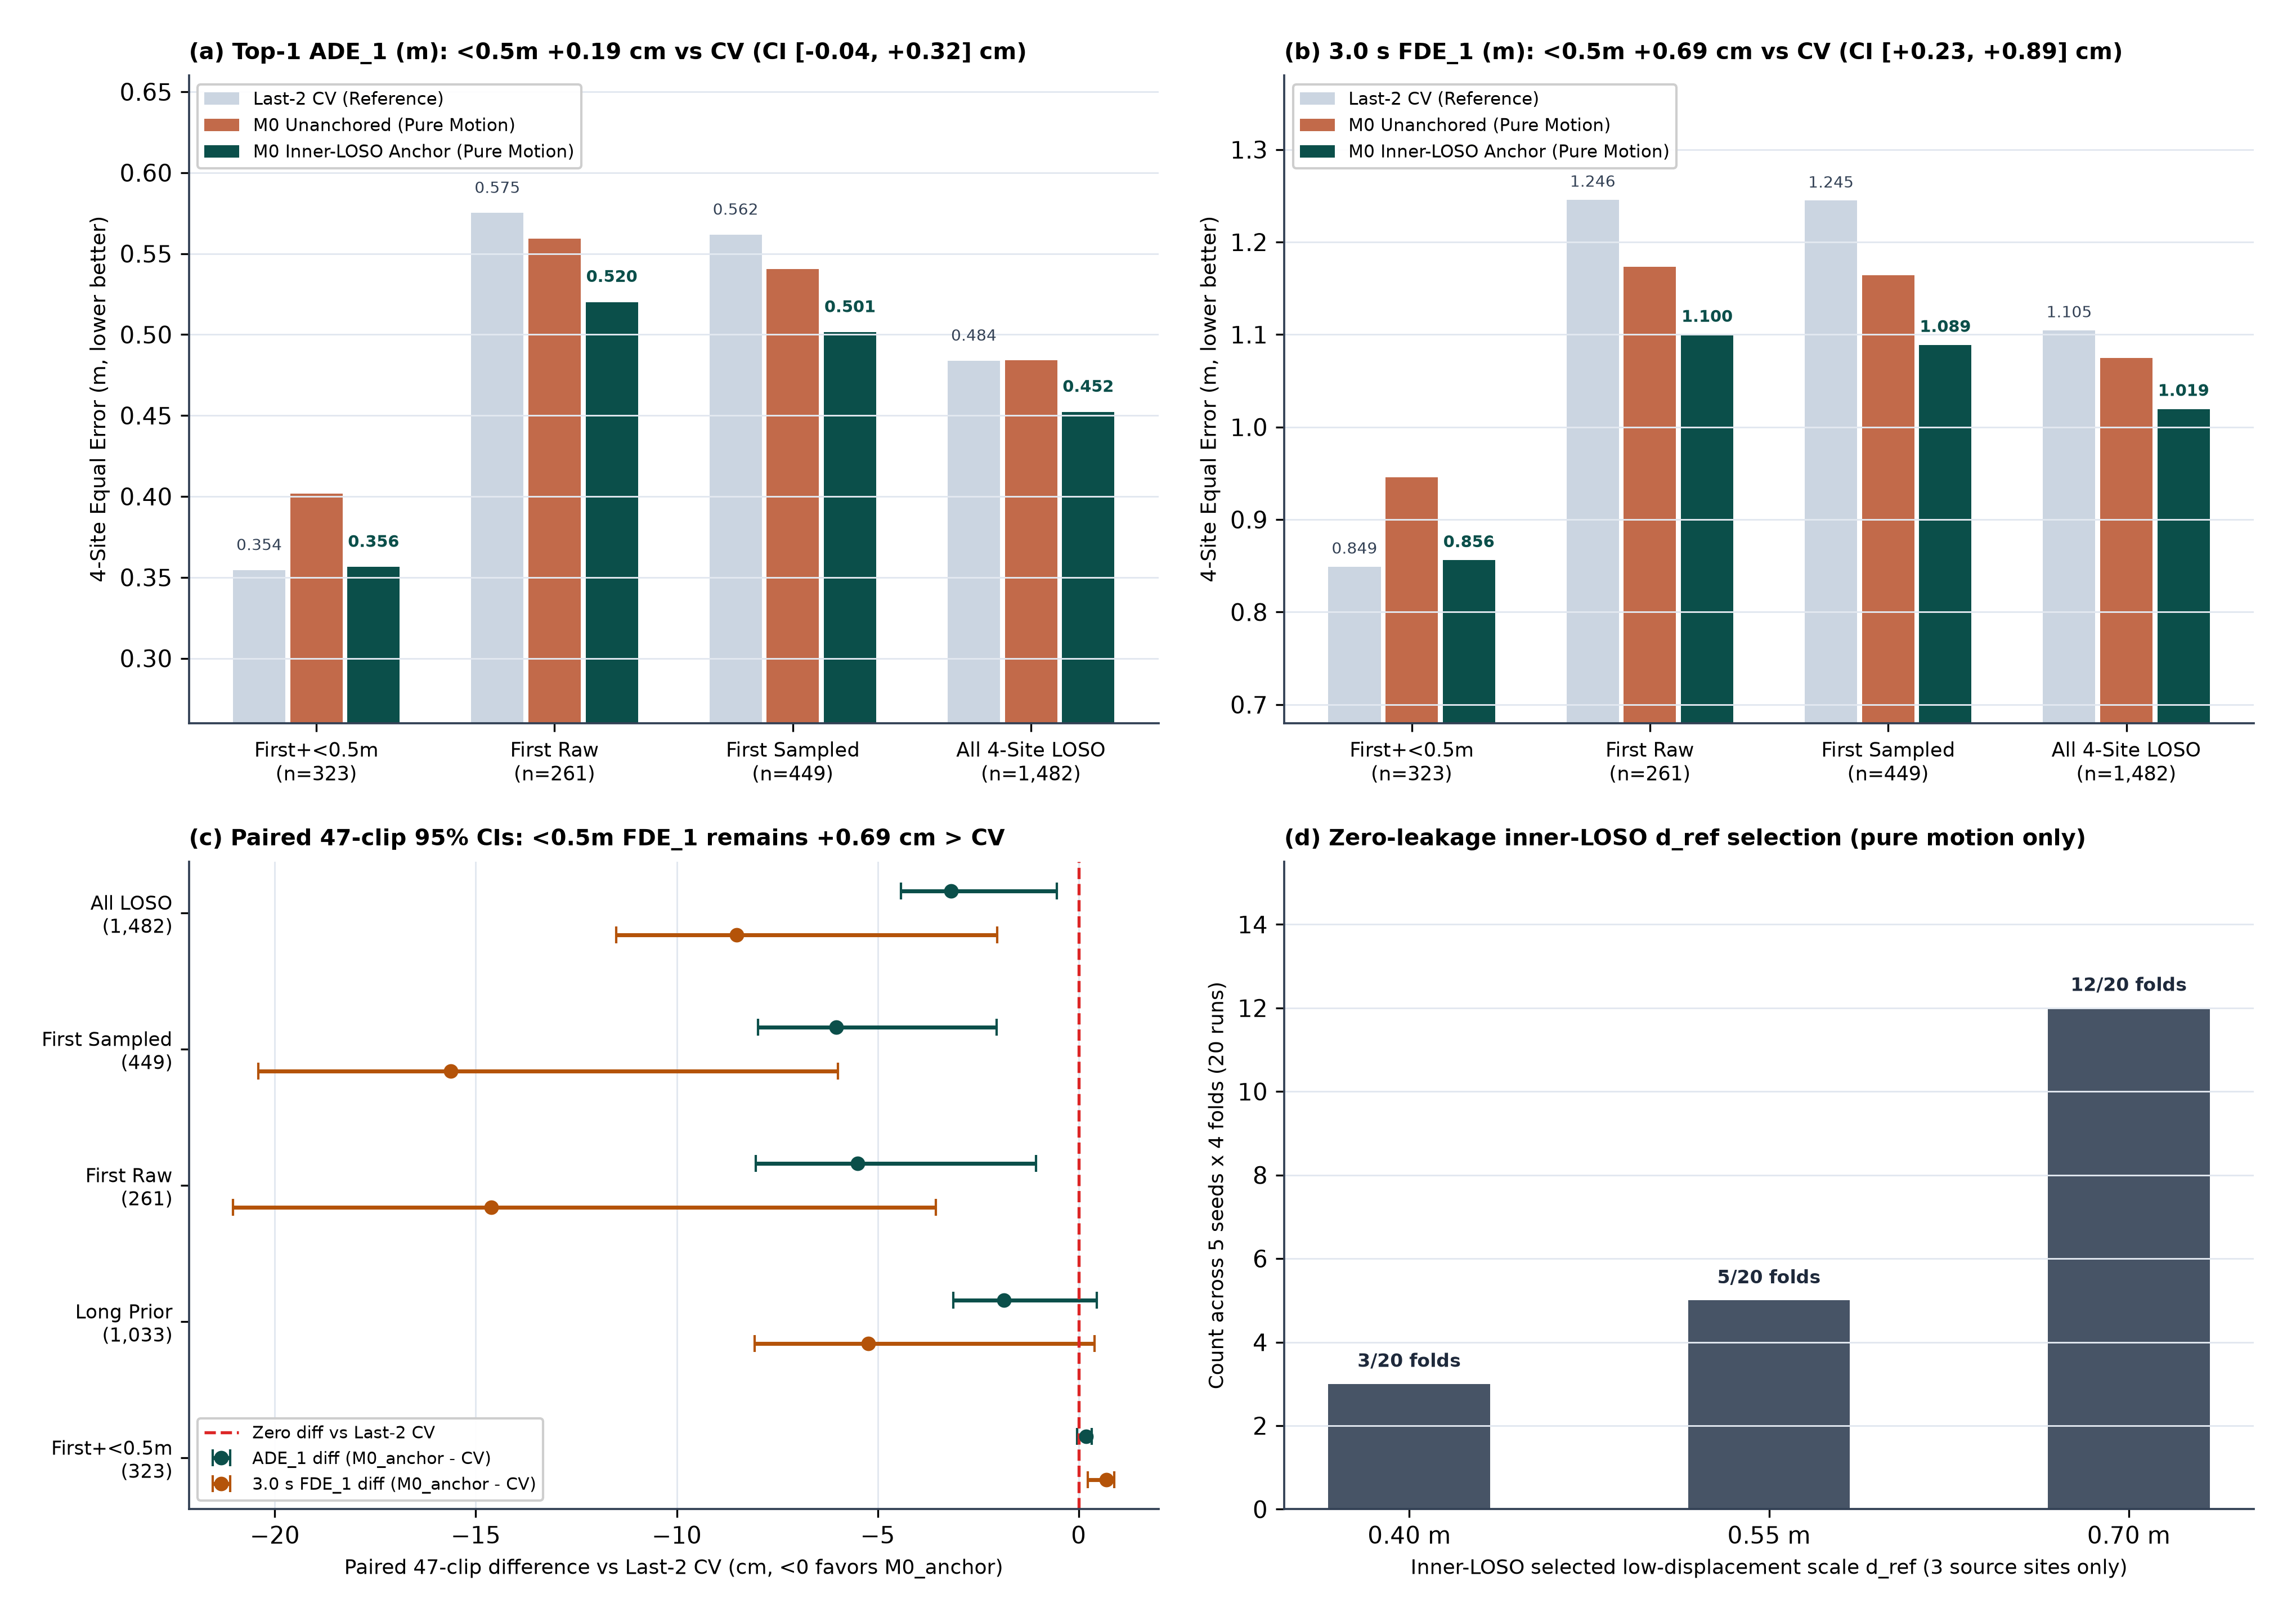
\includegraphics[width=0.95\textwidth]{fig17_ppt_mainline_conformal_and_short_disp.png}
\caption{Controlled $O(2)$ \texttt{M0--M3} ablation, rank-3 homography ground-facing $<0.5\text{ m}$ evaluation, and \texttt{PINNS} fixed-predictor split-conformal coverage.}
\label{fig:m0_m3_conformal}
\end{figure*}

\begin{figure*}[!t]
\centering
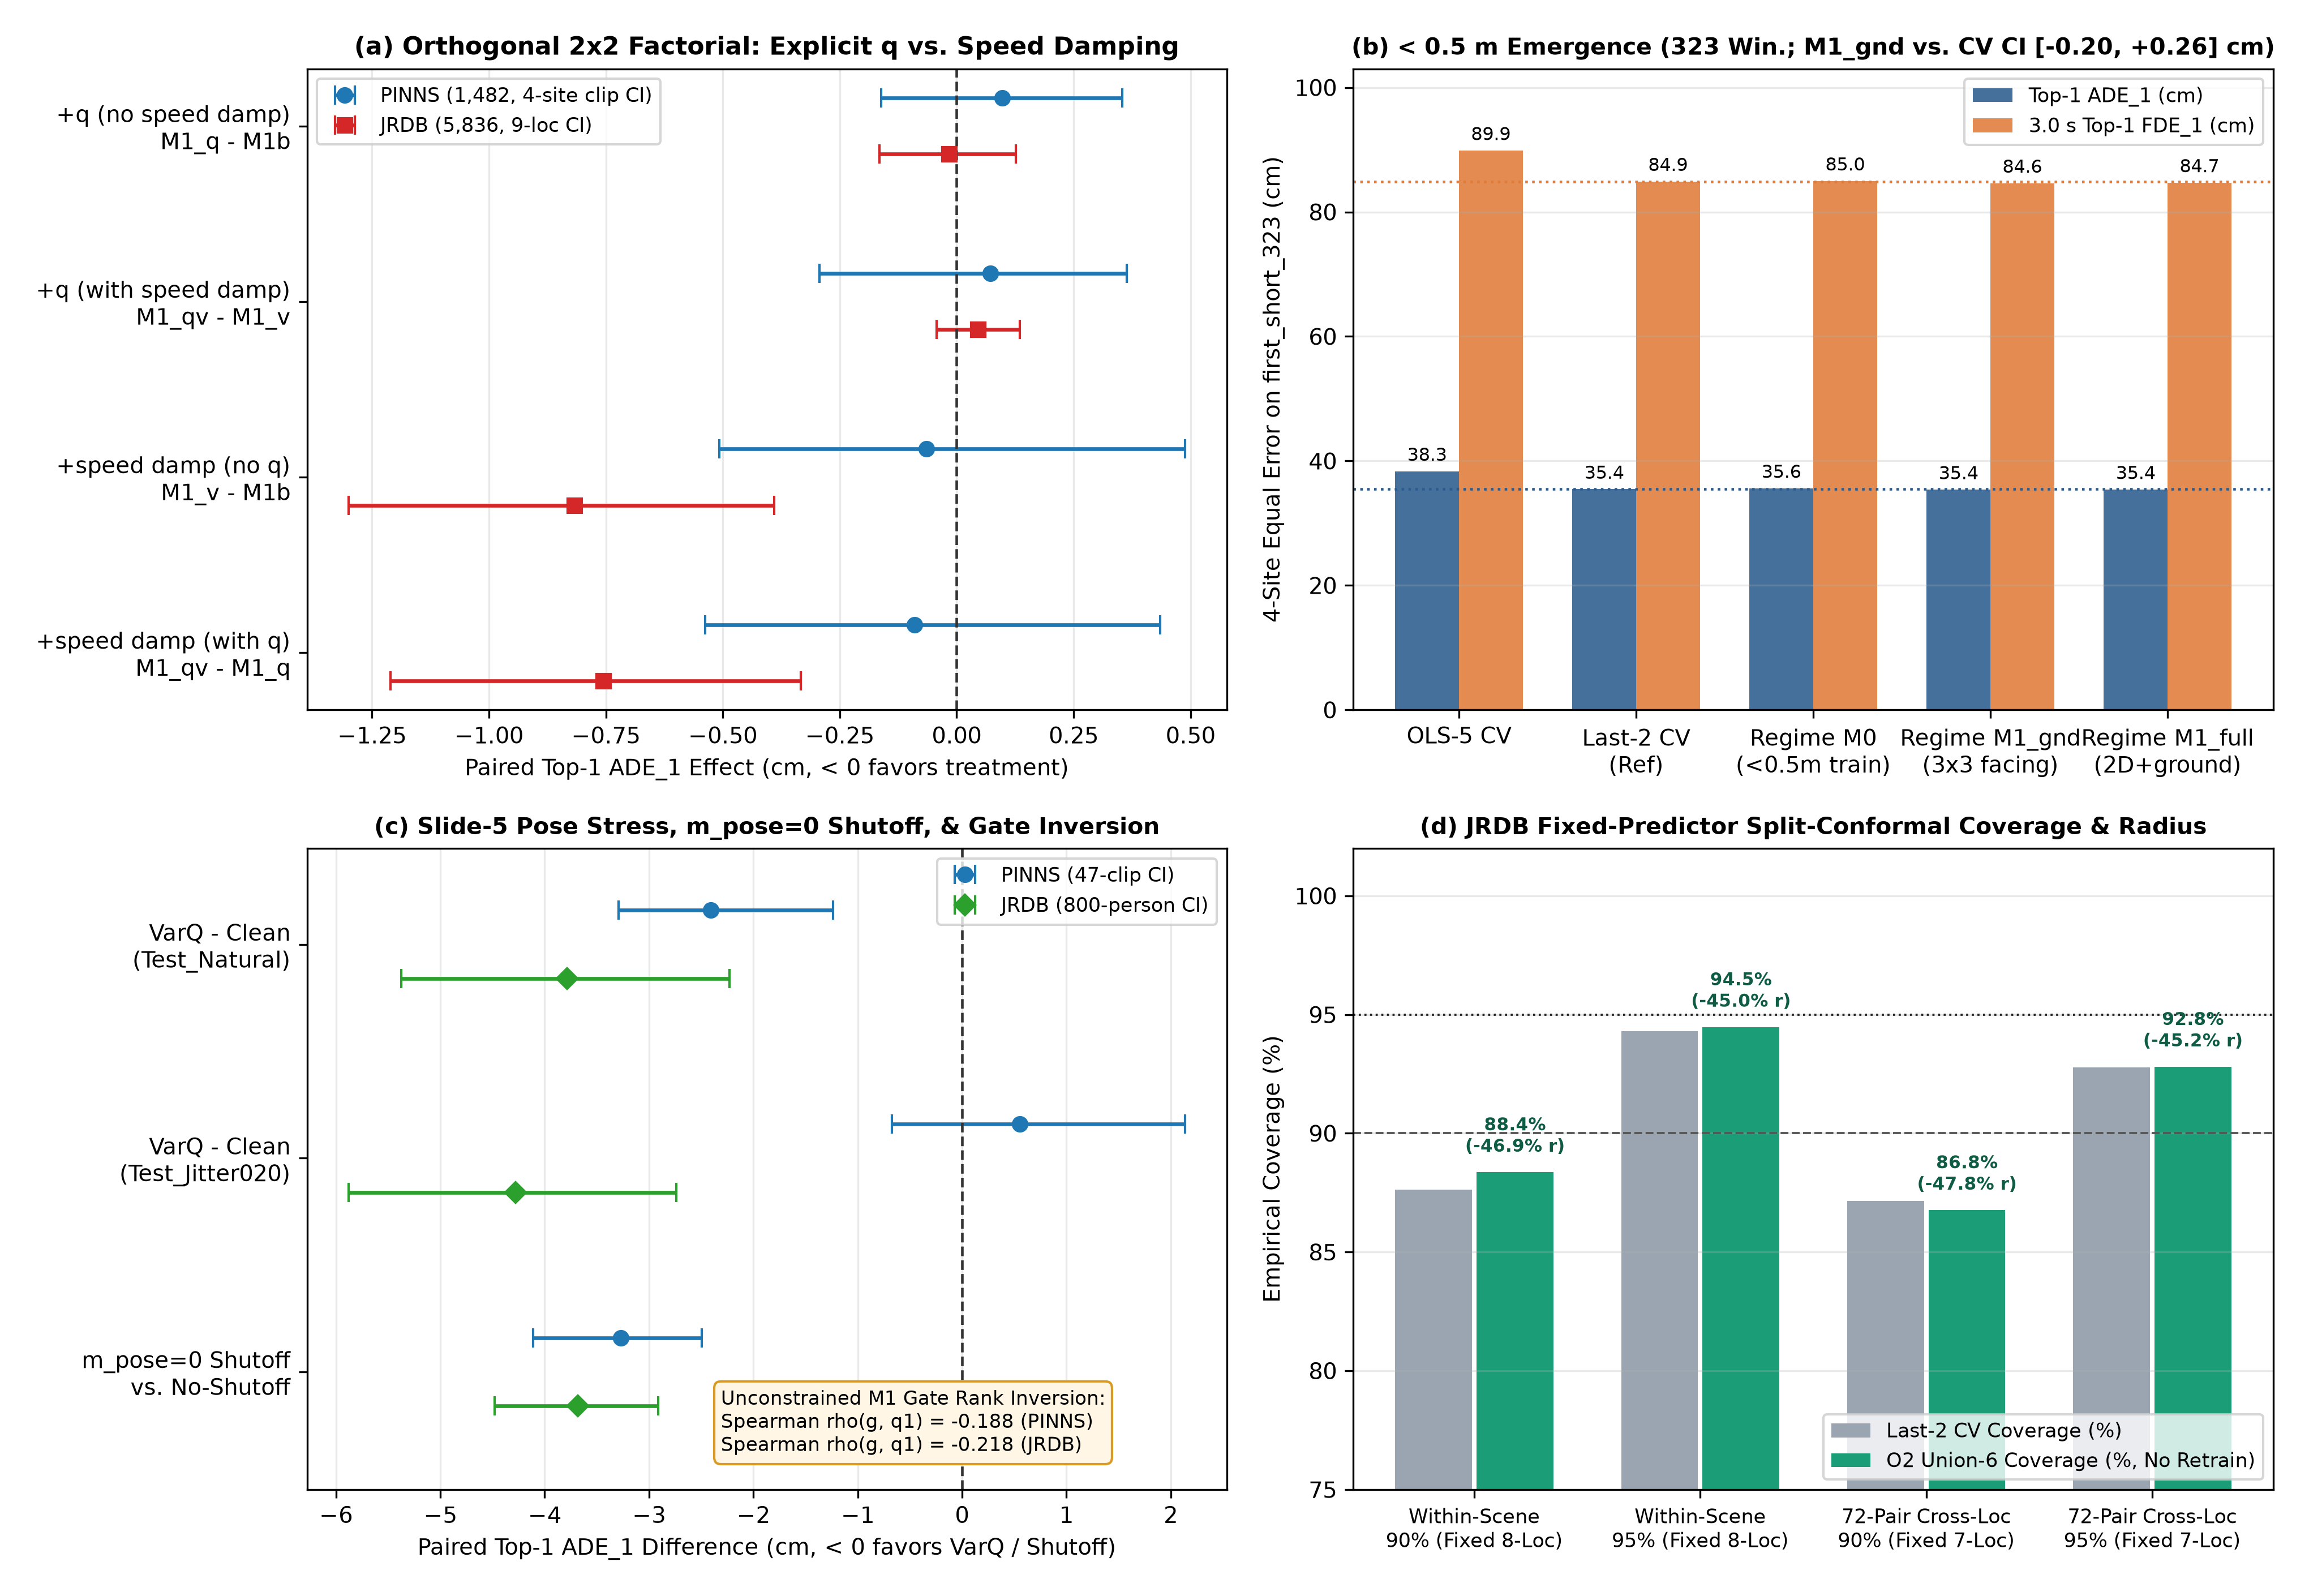
\includegraphics[width=0.95\textwidth]{fig18_wave17_factorial_slide5_and_jrdb_conformal.png}
\caption{Orthogonal $2\times 2$ ($q \times \text{speed}$) factorial, $<0.5\text{ m}$ regime bound, keypoint-degradation and gate rank-inversion audit, and \texttt{JRDB} 72-pair conformal coverage.}
\label{fig:factorial_slide5}
\end{figure*}

\subsection{\texttt{JRDB} 9-Location Chain and Fixed-Predictor Conformal Tubes}
On \texttt{JRDB} ($5{,}836$ windows across $9$ campus locations), \texttt{Last-2 CV} ($0.2812 / 0.5521\text{ m}$) retains the lowest single-mode \texttt{Top-1} $\text{ADE}_1$ (\texttt{O2-M0}: $0.2947 / 0.5739\text{ m}$) due to smooth $2.5\text{ Hz}$ corridor walking. Nevertheless, 6-mode $\text{minFDE}_6$ drops monotonically by $-44.3\%$ along \texttt{CV} $\to$ \texttt{M0} $\to$ \texttt{M1} $\to$ \texttt{M2b} $\to$ \texttt{M3} ($0.5521 \to 0.3369 \to 0.3288 \to 0.3116 \to 0.3078\text{ m}$), radial approaching speed $v_{\text{rad}}$ lowers partial-occlusion $\text{ADE}_1$ by $-0.83\text{ cm}$ ($[-1.92, -0.07]\text{ cm}$), and 5-action supervision ($\text{Macro-AP} = 0.3498$) enables \texttt{M3a}/\texttt{M3b} to beat \texttt{M2b} on \texttt{Top-1} $\text{ADE}_1$ by $-0.80 / -0.78\text{ cm}$ ($[-1.57, -0.20]\text{ cm}$). Table~\ref{tab:split_conformal} confirms strict zero-retrain split-conformal coverage (whereas a legacy retrained empirical check yielded $93.79\% / 96.33\%$ without formal exchangeability).

\begin{table*}[!t]
\centering
\caption{Fixed-Predictor Split-Conformal Safety Coverage and Tube Radius Without Post-Calibration Retraining}
\label{tab:split_conformal}
\footnotesize
\begin{tabular}{lccccc}
\toprule
Benchmark \& Strict Zero-Retrain Protocol & Nominal $1-\alpha$ & \texttt{Last-2 CV} Cov.\ / Rad.\ (m) & \texttt{O2-M3} \texttt{Top-1} Cov. & \texttt{O2-M3} (\texttt{M2b}) \texttt{Union-6} Cov.\ / Rad.\ (m) & Radius vs.\ \texttt{CV} \\
\midrule
\texttt{PINNS} Within-Site 50/50 Clip Split (Fixed 3-Site) & 90\% / 95\% & 90.35\% (2.655) / 95.33\% (3.751) & 89.99\% / 95.02\% & \textbf{90.60\% (1.593) / 94.94\% (2.384)} & \textbf{$-40.0\% / -36.4\%$} \\
\texttt{PINNS} Cross-Country 12 Pairs (Fixed 2-Site) & 90\% / 95\% & 87.31\% (2.704) / 92.22\% (3.816) & 87.24\% / 92.33\% & \textbf{86.48\% (1.632) / 91.74\% (2.428)} & \textbf{$-39.6\% / -36.4\%$} \\
\texttt{JRDB} Within-Scene Temporal Split (Fixed 8-Loc) & 90\% / 95\% & 87.62\% (1.364) / 94.31\% (1.912) & 88.99\% / 94.64\% & \textbf{88.37\% (0.724) / 94.48\% (1.051)} & \textbf{$-46.9\% / -45.0\%$} \\
\texttt{JRDB} Cross-Location 72 Pairs (Fixed 7-Loc) & 90\% / 95\% & 87.14\% (1.426) / 92.77\% (1.928) & 86.30\% / 92.81\% & \textbf{86.77\% (0.744) / 92.81\% (1.056)} & \textbf{$-47.8\% / -45.2\%$} \\
\bottomrule
\end{tabular}
\end{table*}

\subsection{Causal Radial-Conflict Gating and Zero-Leakage Action Reranking}
Table~\ref{tab:conflict_rerank} shows that receding/distant traffic perturbs un-gated \texttt{PINNS} mode logits ($+2.57\text{ cm}$ on $n=527$ non-approaching windows), whereas \texttt{M2b\_ttc\_conflict\_gate} lowers full-cohort \texttt{PINNS} $\text{ADE}_1 / \text{FDE}_1$ to $0.4572 / 1.0223\text{ m}$ ($-2.45\text{ cm}$ vs.\ un-gated \texttt{M2b}, $-1.96\text{ cm}$ under $\text{TTC} \le 4\text{ s}$) and inner-fold Platt calibration cuts 5-action ECE $4.9\times\text{--}23.6\times$.

\begin{table*}[!t]
\centering
\caption{Causal Radial-Conflict Gating (\texttt{M2b\_ttc\_conflict\_gate}) and Zero-Leakage Action Calibration / Reranking (5 Seeds)}
\label{tab:conflict_rerank}
\footnotesize
\begin{tabular}{lccl}
\toprule
Evaluation Stratum / Metric & \texttt{PINNS} ($n = 1{,}482$, 4-Site LOSO) & \texttt{JRDB} ($n = 5{,}836$, 9-Loc LOLO) & Paired 95\% Clip / Location CI \& Boundary Note \\
\midrule
\texttt{S1\_non\_approaching} (\texttt{M2b\_frozen} $-$ \texttt{M1}) & $+2.57 / +4.43\text{ cm}$ ($n = 527$) & $+0.02 / -0.42\text{ cm}$ ($n = 2{,}860$) & Distant traffic perturbs un-gated logits ($[+0.90, +5.81]\text{ cm}$) \\
All Windows: \texttt{M2b\_ttc\_conflict\_gate} & \textbf{0.4572 / 1.0223 m} (\texttt{M1}: 0.4679 / 1.0424) & \textbf{0.2987 / 0.5806 m} (\texttt{M2b}: 0.3036) & \texttt{PINNS} vs.\ \texttt{M1}: $[-1.52, -0.58]\text{ cm}$; \texttt{JRDB} vs.\ \texttt{M2b}: $[-0.93, -0.05]$ \\
Close Conflict ($\text{TTC} \le 4\text{ s}$ / $d \le 6\text{ m}$) & \textbf{$-1.96 / -3.56\text{ cm}$} vs.\ \texttt{M1} ($\text{TTC} \le 4\text{ s}$) & \textbf{$-0.71 / -1.79\text{ cm}$} vs.\ \texttt{M1} ($d \le 6\text{ m}$) & \texttt{PINNS} CI $[-2.78, -0.60]\text{ cm}$; Car-Approach ($315$): $-1.98\text{ cm}$ \\
5-Action ECE (\texttt{Raw 0.5} $\to$ \texttt{Inner Platt}) & \textbf{0.1717 $\to$ 0.0349} ($\text{F1}$: \textbf{0.3911}) & \textbf{0.0933 $\to$ 0.0040} ($\text{AP}$: \textbf{0.3567}) & Cuts \texttt{PINNS} \texttt{Left}/\texttt{Right} FPs from $236/231$ to $76/46$ \\
Action-Consistent \texttt{Top-1} Reranking (\texttt{M3}) & $0.4810 \to 0.4769\text{ m}$ ($-0.41\text{ cm}$) & \textbf{$0.2973 \to 0.2930\text{ m}$} ($-0.43\text{ cm}$) & \texttt{JRDB} CI $[-0.66, -0.25]\text{ cm}$ (\texttt{PINNS} CI $[-0.96, +0.14]$ crosses zero) \\
\bottomrule
\end{tabular}
\end{table*}

\subsection{External Baselines (\texttt{Raw} vs.\ \texttt{SO(2) Frenet}) and \texttt{Tesla T4} Efficiency}
Table~\ref{tab:ext_t4} benchmarks \texttt{MCENET}~\cite{cheng2020mcenet}, \texttt{HST}~\cite{salzmann2023hst}, and \texttt{Social-Transmotion}~\cite{saadatnejad2024transmotion} in native scene coordinates (\texttt{Raw}) and equipped with our causal \texttt{SO(2) Frenet} canonicalization, alongside CUDA-event synchronized \texttt{Tesla T4} latency ($40$ warm-up + $200$ passes at $B=1, 12$; Fig.~\ref{fig:wave18_pareto}). Raw scene-axis baselines collapse on cross-country \texttt{PINNS} ($0.7808\text{--}0.8792\text{ m}$); even after adding \texttt{SO(2) Frenet}, \texttt{O2-M2b} ($0.4817\text{ m}$; $0.4572\text{ m}$ with conflict gating) beats \texttt{MCENET+Frenet}, \texttt{HST+Frenet}, and \texttt{Social-Transmotion+Frenet} by $-9.17\text{ cm}$ ($[-11.13, -6.12]$), $-6.81\text{ cm}$ ($[-8.81, -4.45]$), and $-14.00\text{ cm}$ ($[-16.54, -11.68]$), while cutting $B=12$ FLOPs by $192\times\text{--}396\times$ ($23.48\text{ MiB}$ peak VRAM).

\begin{table*}[!t]
\centering
\caption{Cross-Scene External Baselines (\texttt{Raw} vs.\ \texttt{SO(2) Frenet}) and Real-Hardware \texttt{Tesla T4} Efficiency (5 Seeds)}
\label{tab:ext_t4}
\footnotesize
\begin{tabular}{lccccccc}
\toprule
Architecture \& Frame & Params & $B{=}12$ MFLOPs & T4 $B{=}1$ $P_{50}/P_{95}$ (ms) & T4 $B{=}12$ $P_{50}/P_{95}$ (ms) & \texttt{PINNS} $\text{ADE}_1 / \text{FDE}_1$ (m) & \texttt{PINNS} $\text{minFDE}_6$/Cross. & \texttt{JRDB} $\text{ADE}_1 / \text{FDE}_1$ (m) \\
\midrule
\texttt{Last-2 CV} (Zero-Param) & 0 & --- & --- & --- & 0.4839 / 1.1046 & 1.1046 / 2.01\% & \textbf{0.2812 / 0.5521} \\
\texttt{Ext1\_MCENET} (\texttt{Raw}) & 216,067 & 299.44 & 5.883 / 7.544 & 6.058 / 10.063 & 0.8052 / 1.5950 & 0.8103 / 3.27\% & 0.4184 / 0.7853 \\
\texttt{Ext1\_MCENET + Frenet} & 216,067 & 299.44 & 5.883 / 7.544 & 6.058 / 10.063 & 0.5734 / 1.1611 & 0.6711 / 2.96\% & 0.3217 / 0.6076 \\
\texttt{Ext2\_HST} (\texttt{Raw}) & 508,483 & 617.57 & 5.271 / 5.741 & 5.755 / 6.353 & 0.7808 / 1.5285 & 0.7835 / 3.47\% & 0.4183 / 0.7695 \\
\texttt{Ext2\_HST + Frenet} & 508,483 & 617.57 & 5.271 / 5.741 & 5.755 / 6.353 & 0.5498 / 1.1213 & 0.6651 / 2.51\% & 0.3243 / 0.6083 \\
\texttt{Ext3\_SocialTransmotion} (\texttt{Raw}) & 517,187 & 383.86 & 5.554 / 6.147 & 5.577 / 6.126 & 0.8792 / 1.7085 & 0.8332 / 3.56\% & 0.5451 / 0.9872 \\
\texttt{Ext3\_SocialTransmotion + Frenet} & 517,187 & 383.86 & 5.554 / 6.147 & 5.577 / 6.126 & 0.6217 / 1.2348 & 0.6710 / 2.82\% & 0.3541 / 0.6545 \\
\texttt{O2-M0} (Pure Motion) & 27,999 & \textbf{0.17} & \textbf{2.632 / 2.852} & \textbf{2.752 / 3.135} & 0.4618 / 1.0310 & 0.6843 / 1.83\% & 0.2961 / 0.5769 \\
\texttt{O2-M1\_mono\_q} (Monotonic Gate) & 28,005 & 0.32 & 3.362 / 3.769 & 3.506 / 4.025 & 0.4645 / 1.0340 & --- & 0.3024 / 0.5901 \\
\texttt{O2-M2b\_conflict\_gate} (Ours) & 27,999 & 1.56 & 4.855 / 5.329 & 4.782 / 5.231 & \textbf{0.4572 / 1.0223} & 0.6663 / --- & 0.2987 / 0.5806 \\
\texttt{O2-M3 / M3a} (5-Action Bridge) & 27,999 & 9.47 & 6.516 / 7.151 & 6.323 / 7.133 & 0.4810 / 1.0628 & \textbf{0.6521} / 2.28\% & 0.2950 / 0.5688 \\
\texttt{Ours\_O2\_Full} (Compact) & \textbf{20,739} & 1.42 & 4.162 / 4.640 & 4.345 / 4.885 & 0.4582 / 1.0096 (Bayes) & --- & --- \\
\bottomrule
\end{tabular}
\end{table*}

\begin{figure*}[!t]
\centering
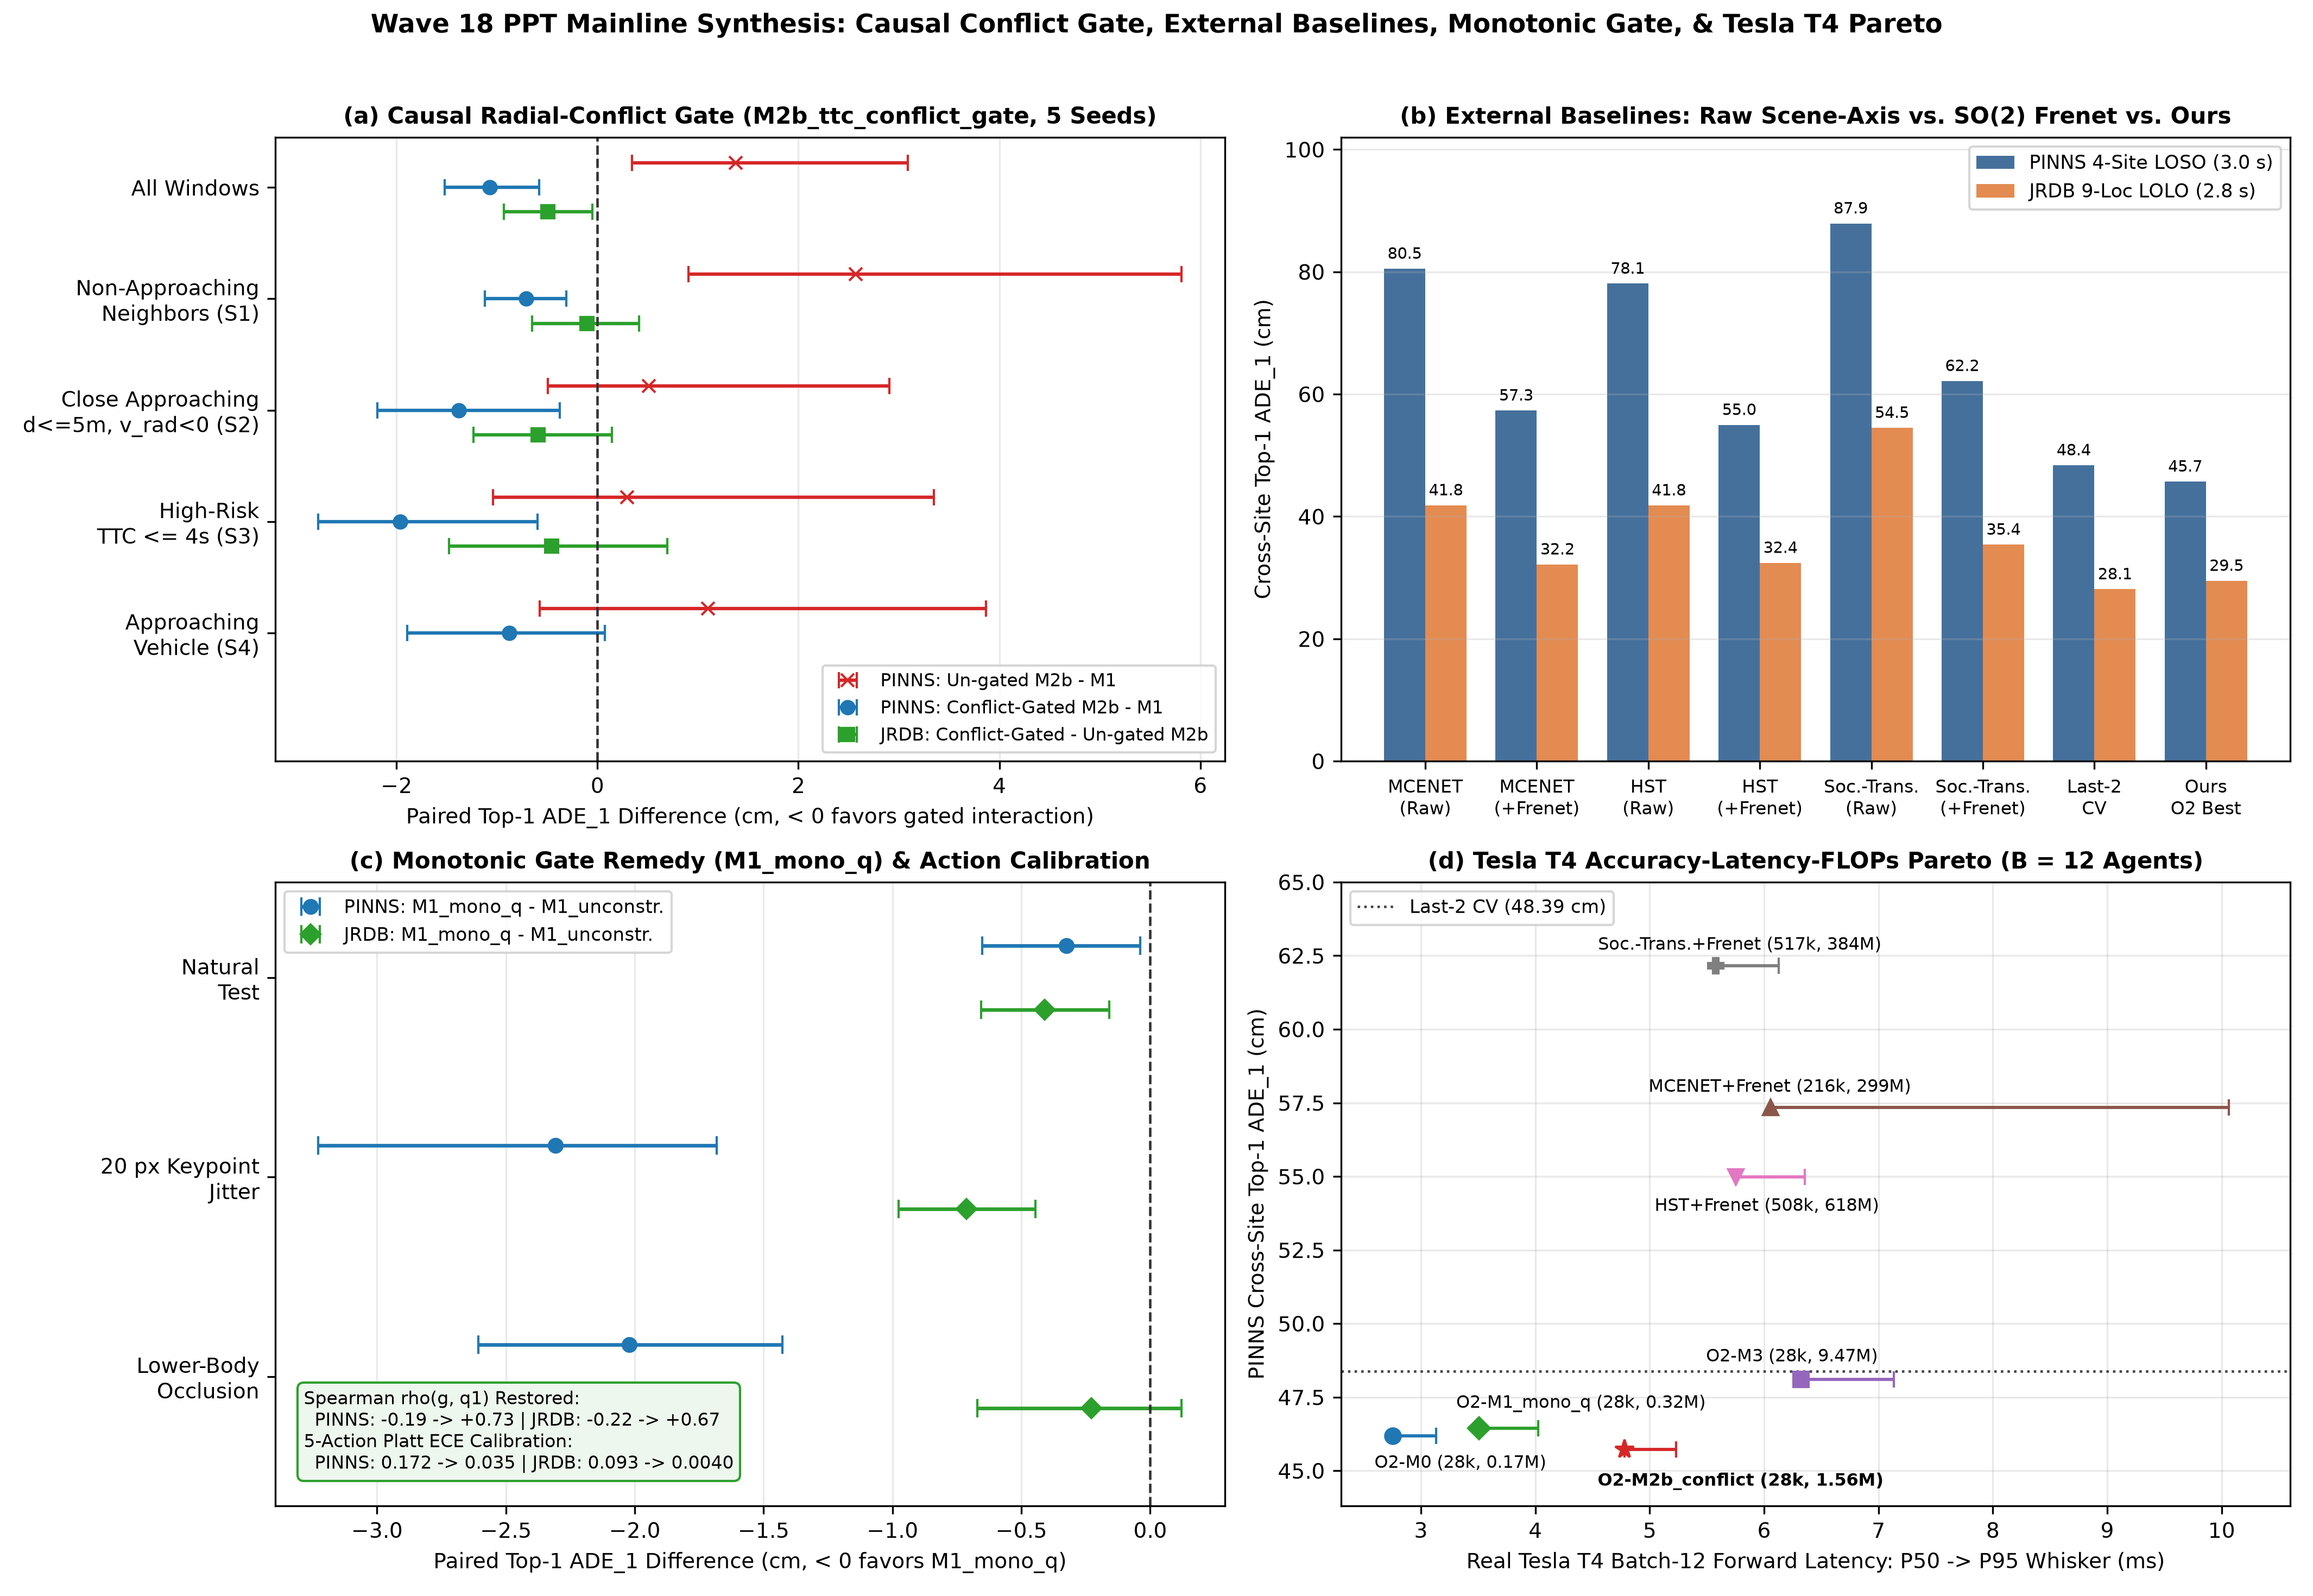
\includegraphics[width=0.95\textwidth]{fig19_wave18_conflict_rerank_ext_and_t4_pareto.png}
\caption{Causal radial-conflict gate, cross-scene external baselines (\texttt{Raw} vs.\ \texttt{SO(2) Frenet}), structurally monotonic quality gate, and real-hardware \texttt{Tesla T4} Pareto frontier.}
\label{fig:wave18_pareto}
\end{figure*}

\subsection{Unified Remediated Chain and Zero-Shot \texttt{DUT / IMPTC} Transfer}
Table~\ref{tab:unified_transfer} evaluates stacking all architectural remedies into a single polylineless chain (\texttt{U\_M0} $\to$ \texttt{U\_M1\_mono} $\to$ \texttt{U\_M2b\_mono\_conflict} $\to$ \texttt{U\_M3\_mono\_conflict}) alongside zero-shot transfer of the \texttt{PINNS} 5-seed ensemble ($0.0\text{ m}$ 5-axis $O(2)$ swing) to \texttt{DUT} ($3{,}066$ windows) and \texttt{IMPTC} ($564$ windows) with zero target-domain training. On \texttt{PINNS}, \texttt{U\_M2b\_mono\_conflict} reaches $0.4510 / 1.0097\text{ m}$ ($-5.50 / -16.16\text{ cm}$ vs.\ \texttt{CV} on $\text{TTC} \le 4\text{ s}$), whereas co-adapting shared trajectory knots under multi-task BCE on $\sim 1{,}100$-window folds incurs $+2.04\text{ cm}$ (\texttt{U\_M3}), contrasting with larger \texttt{JRDB} folds ($\sim 5{,}180$ windows) where \texttt{U\_M3\_rerank} drops $\text{ADE}_1 / \text{FDE}_1$ to $0.2917 / 0.5638\text{ m}$ ($\text{ECE} = 0.0053$). Zero-shot \texttt{M2b\_ttc\_conflict\_gate} lowers \texttt{DUT} car-approaching error by $-6.98 / -13.84\text{ cm}$ vs.\ un-gated \texttt{M2b\_frozen} and delivers $89.76\% / 95.50\%$ (\texttt{DUT} 72-pair) and $89.51\% / 94.21\%$ (\texttt{IMPTC} 12-pair) zero-retrain \texttt{Union-6} coverage.

\begin{table*}[!t]
\centering
\caption{Unified Remediated $O(2)$ Chain (\texttt{PINNS} \& \texttt{JRDB}) and Zero-Shot Conflict-Gated \& Split-Conformal Transfer (\texttt{DUT} \& \texttt{IMPTC}, 5 Seeds)}
\label{tab:unified_transfer}
\footnotesize
\begin{tabular}{llll}
\toprule
Benchmark \& Protocol & Key Model Comparison ($\text{ADE}_1 / \text{FDE}_1$ m; $\text{minFDE}_6$) & Paired 95\% Cluster CI ($\text{ADE}_1$) & Zero-Retrain \texttt{Union-6} ($90\% / 95\%$ Cov.; Rad.) \\
\midrule
\texttt{PINNS} Unified ($1{,}482$, $\rho_{q_1}{=}{+0.8149}$) & \textbf{\texttt{U\_M2b}: 0.4510 / 1.0097} (0.6563) vs.\ \texttt{CV} 0.4839 / 1.1046 & vs.\ \texttt{CV}: $[-4.76, -0.18]\text{ cm}$ & Within-site: 88.78\% / 93.41\% ($-44.5\% / -36.5\%$) \\
\texttt{JRDB} Unified ($5{,}836$, $\rho_{q_1}{=}{+0.8429}$) & \textbf{\texttt{U\_M3\_rerank}: 0.2917 / 0.5638} (0.3143; ECE 0.0053) & vs.\ \texttt{U\_M3}: $[-0.37, -0.18]\text{ cm}$ & Within-loc: 88.48\% / 95.20\% ($-46.0\% / -41.2\%$) \\
\texttt{DUT} Zero-Shot ($3{,}066$, Swing $0.0\text{ m}$) & \textbf{\texttt{M2b\_conflict}: 0.6096 / 1.2859} (0.7066; \texttt{M2b}: 0.6475) & vs.\ \texttt{M2b}: $[-5.92, -1.78]\text{ cm}$ & \textbf{72 Cross-Clip}: \textbf{89.76\% / 95.50\%} ($-31.2\% / -29.0\%$) \\
\texttt{IMPTC} Zero-Shot ($564$, Swing $0.0\text{ m}$) & \textbf{\texttt{M2b\_conflict}: 0.2413 / 0.5923} (0.3729; \texttt{M2b}: 0.2559) & vs.\ \texttt{M2b}: $[-2.22, -0.79]\text{ cm}$ & \textbf{12 Cross-Seq}: \textbf{89.51\% / 94.21\%} ($-38.7\% / -37.7\%$) \\
\bottomrule
\end{tabular}
\end{table*}

\subsection{Decoupled Synergy, Usable-Pose Threshold, and Adaptive Conformal}
Three targeted audits close the remaining architectural and safety questions (Fig.~\ref{fig:wave19_20}):
\begin{enumerate}
  \item \textbf{Representation-Decoupled \texttt{M3} Synergy ($0.4505 / 1.0085\text{ m}$ on \texttt{PINNS}):} Freezing \texttt{U\_M2b\_mono\_conflict} knots ($0.0\text{ m}$ drift) while fitting the parity-consistent 5-action head (\texttt{U\_M3\_decoupled\_platt\_rerank}) eliminates the small-fold multi-task penalty ($-2.20 / -4.08\text{ cm}$ vs.\ co-adapted \texttt{U\_M3}, 95\% clip CI $[-2.68, -1.64]\text{ cm}$), achieves our best \texttt{PINNS} $\text{ADE}_1 / \text{FDE}_1$ of $0.4505 / 1.0085\text{ m}$ ($[-4.82, -0.26]\text{ cm}$ vs.\ \texttt{CV}), and raises 5-action $\text{Macro-AP}$ to $0.4051$ ($\text{ECE} = 0.0580$).
  \item \textbf{Minimum Usable Pixel Height and Completeness Boundary:} Below $50\text{ px}$ ($n = 98$) or $q_1 < 0.75$, direct (\texttt{M1a}) and unconstrained (\texttt{M1}) fusion degrade $\text{ADE}_1$ over \texttt{M0} by $+3.05 / +3.70\text{ cm}$ ($<50\text{ px}$) and $+3.81 / +6.15\text{ cm}$ (\texttt{JRDB} $q_1 < 0.75$), whereas \texttt{M1\_mono\_q} throttles $\bar{g}$ ($0.334$ at $<50\text{ px}$, $0.095\text{--}0.110$ at $q_1 < 0.40$), saving $-1.65$ to $-5.28\text{ cm}$. On the true $20$-frame $623$-window $3\times 3$ matrix, \texttt{M1\_mono\_q} restores $\rho(g, q_1)$ to $+0.7930 / +0.8365 / +0.8674$ across $T = 5, 10, 20$ ($-1.37\text{ cm}$ vs.\ \texttt{M1} on $T=5$ Heavy; $-0.71\text{ cm}$ $[-1.63, +0.21]\text{ cm}$ vs.\ \texttt{M0} on $T=20$ Clear, confirming motion sufficiency).
  \item \textbf{Zero-Retrain Locally-Weighted Conformal ($72$-Pair \texttt{JRDB}):} Source-OOF NNLS scaling (\texttt{M3\_speed\_spread\_scaled}, Proposition~3) lifts \texttt{JRDB} $72$-pair cross-location \texttt{Union-6} coverage from $86.81\% / 92.87\%$ to $88.89\% / 94.20\%$ (\texttt{Top-1}: $89.14\% / 94.17\%$), shrinks mean radius to $0.6301 / 0.9146\text{ m}$ ($-55.8\% / -52.5\%$ vs.\ \texttt{CV}), and raises fast-pedestrian ($\ge 1.0\text{ m/s}$) $90\%$ coverage from $75.06\%$ to $89.51\%$ (cutting within-scene speed-stratum gap from $22.01\%$ to $9.30\%$; on 2-site \texttt{PINNS}, constant-radius $86.57\% / 91.70\%$ remains preferable for slow walkers).
\end{enumerate}

\begin{figure*}[!t]
\centering
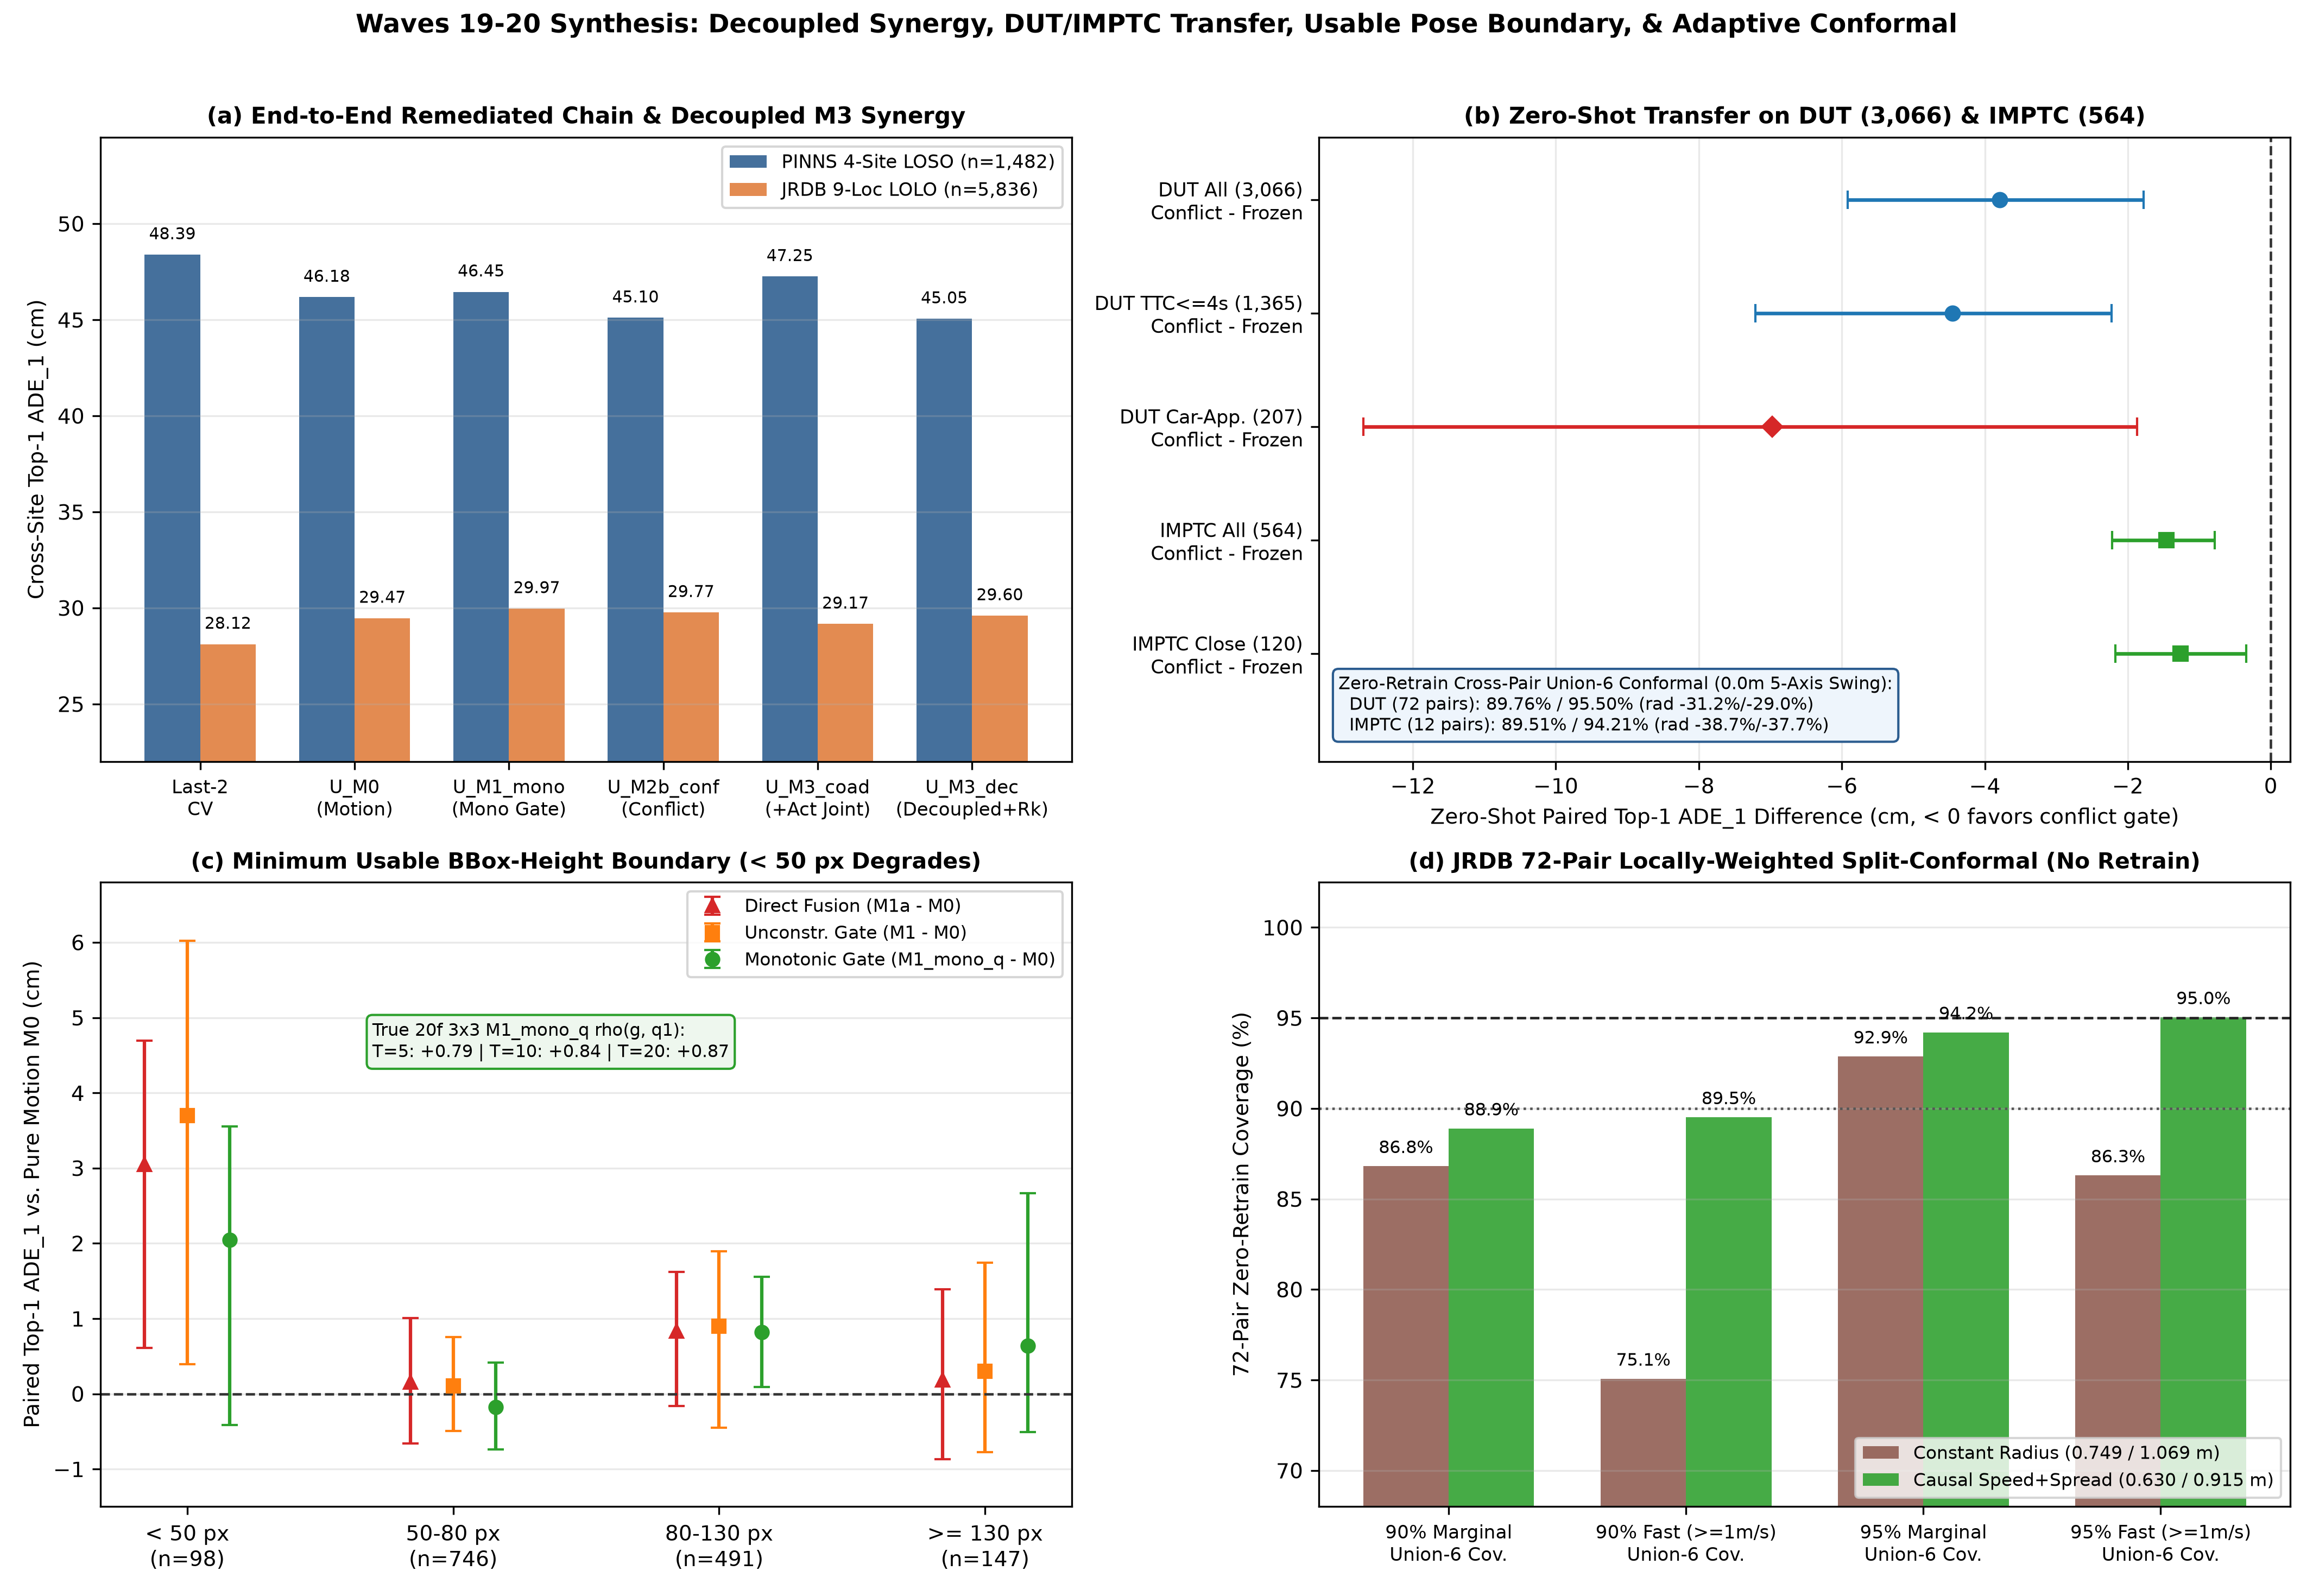
\includegraphics[width=0.95\textwidth]{fig20_wave19_20_unified_dut_boundary_and_adaptive_conformal.png}
\caption{End-to-end remediated chain and decoupled \texttt{M3} synergy, zero-shot \texttt{DUT}/\texttt{IMPTC} transfer, minimum usable bbox-height boundary, and \texttt{JRDB} 72-pair locally-weighted split-conformal calibration.}
\label{fig:wave19_20}
\end{figure*}

\subsection{Raw-Video De-Occlusion Audit, Automatic RTMPose-17 Video Skeletons, Iso-Test-FPR Lead-Time, and Partitioned Benchmarks}
To rigorously test whether 5 frames of pose anticipate \texttt{Start}, \texttt{Stop}, or \texttt{Turn} earlier than ground position right after physical de-occlusion, Table~\ref{tab:wave21_22} and Figs.~\ref{fig:wave21}--\ref{fig:wave22} synthesize Waves 21--23 across four pose-bearing benchmarks and three zero-pose motion/interaction controls:
\begin{enumerate}
  \item \textbf{Camera-Homography Fix, Raw-Video Inspection, \& Conditioned Medoid Selection:} Projecting 3D vehicles into original camera pixels via verified rank-3 homographies ($3.28\times 10^{-5}\text{ px}$ median footpoint error) shows only $1/34$ prior BEV-pixel vehicle flags matched in camera space ($189$ homography candidates). Prediction-blind visual inspection of all $241$ non-Frame-0 \texttt{first\_contiguous} windows across $26$ raw \texttt{ori\_*.mp4} clips confirms $140 / 449$ ($31.2\%$) visual physical occluder emergences ($32$ vehicle, $63$ static portals/pillars, $45$ foreground pedestrians), $27$ border entries, $74$ open-view late pickups, and $208$ ($46.3\%$) Frame-0 clip-start artifacts ($175 / 323 = 54.2\%$ in \texttt{first\_short\_323}). On \texttt{PINNS} \texttt{all\_1482} (\texttt{CV} $0.4839 / 1.1046\text{ m}$, \texttt{S6\_M0} $0.4497 / 1.0048\text{ m}$, \texttt{S6\_M1} $0.4486 / 1.0005\text{ m}$, \texttt{S6\_Full} $0.4472 / 0.9926\text{ m}$), conditioned risk-medoid decoding (\texttt{S6\_Full\_CondMedoid}) sets our new all-time best at $0.4382 / 0.9778\text{ m}$ ($-4.56 / -12.68\text{ cm}$ vs.\ \texttt{CV}, 95\% CI $[-6.34, -1.01]$ / $[-16.91, -4.21]\text{ cm}$). Pure 5-frame pose (\texttt{S6\_M1} $-$ \texttt{S6\_M0}) slightly raises $3.0\text{ s}$ $\text{ADE}_1$ on $189$ emergences ($0.5730 \to 0.5828\text{ m}$; $+1.49\text{ cm}$ on $132$ locked-eval windows), while cutting post-onset $+0.5\text{ s}/+1.0\text{ s}$ error by $-2.17 / -2.19\text{ cm}$ ($[-2.30, -1.58]\text{ cm}$) on emerging maneuvers where $95/107$ ($99/109$ in Wave 21) involve \texttt{Turn} ($-2.12 / -2.13\text{ cm}$ on $95$ \texttt{Turn}-only windows vs.\ $2$ \texttt{Start}, $10$ \texttt{Stop}), supporting short-horizon turning prediction rather than early \texttt{Start} detection. Across all $5$ seeds, \texttt{CondMedoid} generates \texttt{Start} ($9.0/9$) and \texttt{Stop} ($18.0/18$) $100\%$ (\texttt{JRDB}: $11.0/11$, $2.0/2$), whereas Rank-1 selection hits $0.0/9$ \texttt{Start} and $1.8/18$ \texttt{Stop} (\texttt{CondF1Slot}: $5.0/9$ \texttt{Start} at $26.8/39$ false positives).
  \item \textbf{Real Automatic \texttt{RTMPose-17} Skeletons \& Unconflated $5.10\%$ Iso-Test-FPR Lead-Time:} In \texttt{JAAD 2.0}~\cite{kotseruba2017jaad} ($2{,}363$ windows, $953$ locked test in \texttt{bbox\_heights}; low-disp $<0.25$ \texttt{bbox\_heights}), the $406$-window cohort comprises $168$ strict 5-frame de-occlusions (\texttt{full/part->none} at frame 4), $114$ ongoing \texttt{part}, $74$ ongoing \texttt{full}, and $50$ late starts. Extracting real 17-joint \texttt{RTMPose-m} skeletons over $21{,}078$ frames ($317$ videos) separates automatic video pose (\texttt{J\_AutoPose\_rtmpose17}) from human-annotated body orientation + gaze (\texttt{J\_HumanAttr\_orient\_gaze}). On $168$ strict de-occlusions, \texttt{J\_AutoPose\_veh} ($0.5027 / 1.1718$ \texttt{bbox-H}) beats \texttt{CV} ($0.5155 / 1.2031$, $[-0.0270, -0.0009]$) and raises \texttt{Start/Stop/Cross} AP from $0.7389/0.1328/0.4698$ (\texttt{BBox+Veh}) to $0.8998/0.1640/0.5540$ (\texttt{HumanAttr+Veh}: $0.4250 / 1.0461$ on $953$ test, $-17.2\%$ post-onset on $406$). At identical $5.10\%$ realized test FPR ($235$ true negatives, zero miss penalty) on strictly recovered post-de-occlusion events ($12$ \texttt{Start}, $10$ \texttt{Stop}), \texttt{KinOnly} hits $2/12$ \texttt{Start} ($16.7\%$, $10$ missed, $700.0\text{ ms}$ hit lead) and $0/10$ \texttt{Stop} ($0.0\%$), whereas automatic \texttt{RTMPose-17} raises recall to $6/12$ \texttt{Start} ($50.0\%$, $+33.3\%$ $[+8.3\%, +58.3\%]$, $633.3\text{ ms}$ hit lead; \texttt{AutoPose+Veh} $+340.0\text{ ms}$ $[+20.0, +680.0]\text{ ms}$ earlier than \texttt{VehOnly} on $5$ common hits) and $3/10$ \texttt{Stop} ($30.0\%$; $9/38 = 23.7\%$ vs.\ $1/38 = 2.6\%$ on all $38$ test \texttt{Stop}, $+21.1\%$ $[+5.3\%, +36.8\%]$), and fires $+250.0\text{ ms}$ ($[+50.0, +470.0]\text{ ms}$, $n=10$) earlier on \texttt{Start} and $+500.0\text{ ms}$ ($[+342.9, +642.9]\text{ ms}$, $n=14$) earlier on \texttt{Cross} than \texttt{KinOnly} across all test common hits.
  \item \textbf{Two-Rule Automated Barrier Filter:} Clip-polyline union restores lines in $350 / 835$ windows, and our two-rule automated geometric \& causal-trajectory filter ($\kappa_{\text{rule}} = 0.8731$, automated rule concordance) cuts GT crossings from $2.36\%$ to $0.27\%$, yet \texttt{No\_Map} ($0.4919\text{ m}$) still beats \texttt{Fixed\_Auto} ($0.5118\text{ m}$) and \texttt{TwoRule\_Solid} ($0.5069\text{ m}$).
\end{enumerate}

\begin{table*}[!t]
\centering
\caption{Partitioned Seven-Benchmark Evaluation: Four Pose-Bearing Cohorts vs.\ Three Zero-Pose Controls (5 Seeds, Exact Units \& Iso-Test-FPR)}
\label{tab:wave21_22}
\footnotesize
\begin{tabular}{lllll}
\toprule
Benchmark \& Unit & Split / De-Occl Cohort & Primary $\text{ADE}_1 / \text{FDE}_1$ (\texttt{CV} Ref) & Post-Onset Pose / Interaction Gain & 5-Seed Gen \& Exact $5.10\%$-FPR Audit \\
\midrule
\multicolumn{5}{l}{\textit{Part A: Pose-Bearing Benchmarks (2D/3D Automatic Video Skeletons or Human Attributes)}} \\
\texttt{PINNS} (m) & $1{,}482$ / $140$ Vis ($189$ Hom) & \textbf{0.4382 / 0.9778} (\texttt{CV} 0.4839) & Turn-Dom ($107$) Pose: \textbf{$-2.17 / -2.19\text{ cm}$} & \texttt{Start/Stop} Gen \textbf{100\%} (Sel 0/9, 1.8/18) \\
\texttt{JAAD 2.0} (bbox-H) & $953$ Test / $168$ Strict De-Occl & Auto \textbf{0.5027} (\texttt{CV} 0.5155); Hum \textbf{0.4250} & Strict Auto AP \textbf{0.900}; Broad Hum \textbf{$-17.2\%$} & Auto Recall \textbf{50\%/30\%}; Common \textbf{+250/+500 ms} \\
\texttt{JRDB} (m) & $5{,}836$ / $507$ De-Occl & \texttt{CondMed} \textbf{0.2764}; \texttt{M2b} \textbf{0.2772} (\texttt{CV} 0.2812) & De-Occl 3D Pose: \textbf{$-0.22 / -0.25\text{ cm}$} & \texttt{Start} $11/11$, \texttt{Stop} $2/2$ Gen \textbf{100\%} \\
\texttt{JTA-228} (m) & $1{,}267$ Locked Test & \texttt{M1} \textbf{0.5564 / 1.1214} (\texttt{M0} 0.5602, \texttt{CV} 0.5659) & Test Pure 3D Pose: \textbf{$-0.38\text{ cm}$} $\text{ADE}_1$ & Iso-$5.10\%$ \texttt{Stop} Recall $20.0\% \to 33.8\%$ \\
\midrule
\multicolumn{5}{l}{\textit{Part B: Zero-Pose Motion \& Interaction Control Benchmarks ($m_{\text{pose}} \equiv 0$ Identically Verified)}} \\
\texttt{ETH/UCY}~\cite{pellegrini2009eth} (m) & $4{,}187$ (5 Scenes, $0$ Pose) & \texttt{Full} 0.3919 $>$ \texttt{CV} \textbf{0.3892} ($+0.27\text{ cm}$) & Active Maneuvers: \textbf{$-9.11 / -11.08\text{ cm}$} & $0.0\text{ cm}$ pose-branch leak verified \\
\texttt{DUT} + \texttt{IMPTC} (m) & $3{,}066$ ($400$ $<0.5$m) + $564$ ($365$) & \texttt{DUT} \textbf{0.3483} (\texttt{CV} 0.5067); \texttt{IMPTC} \textbf{0.2061} (0.2337) & \texttt{IMPTC} $<0.5$m: 0.2126 $\to$ \textbf{0.1942} / 0.2004 & Zero-shot $O(2)$ $0.0\text{ m}$ swing verified \\
\bottomrule
\end{tabular}
\end{table*}

\begin{figure*}[!t]
\centering
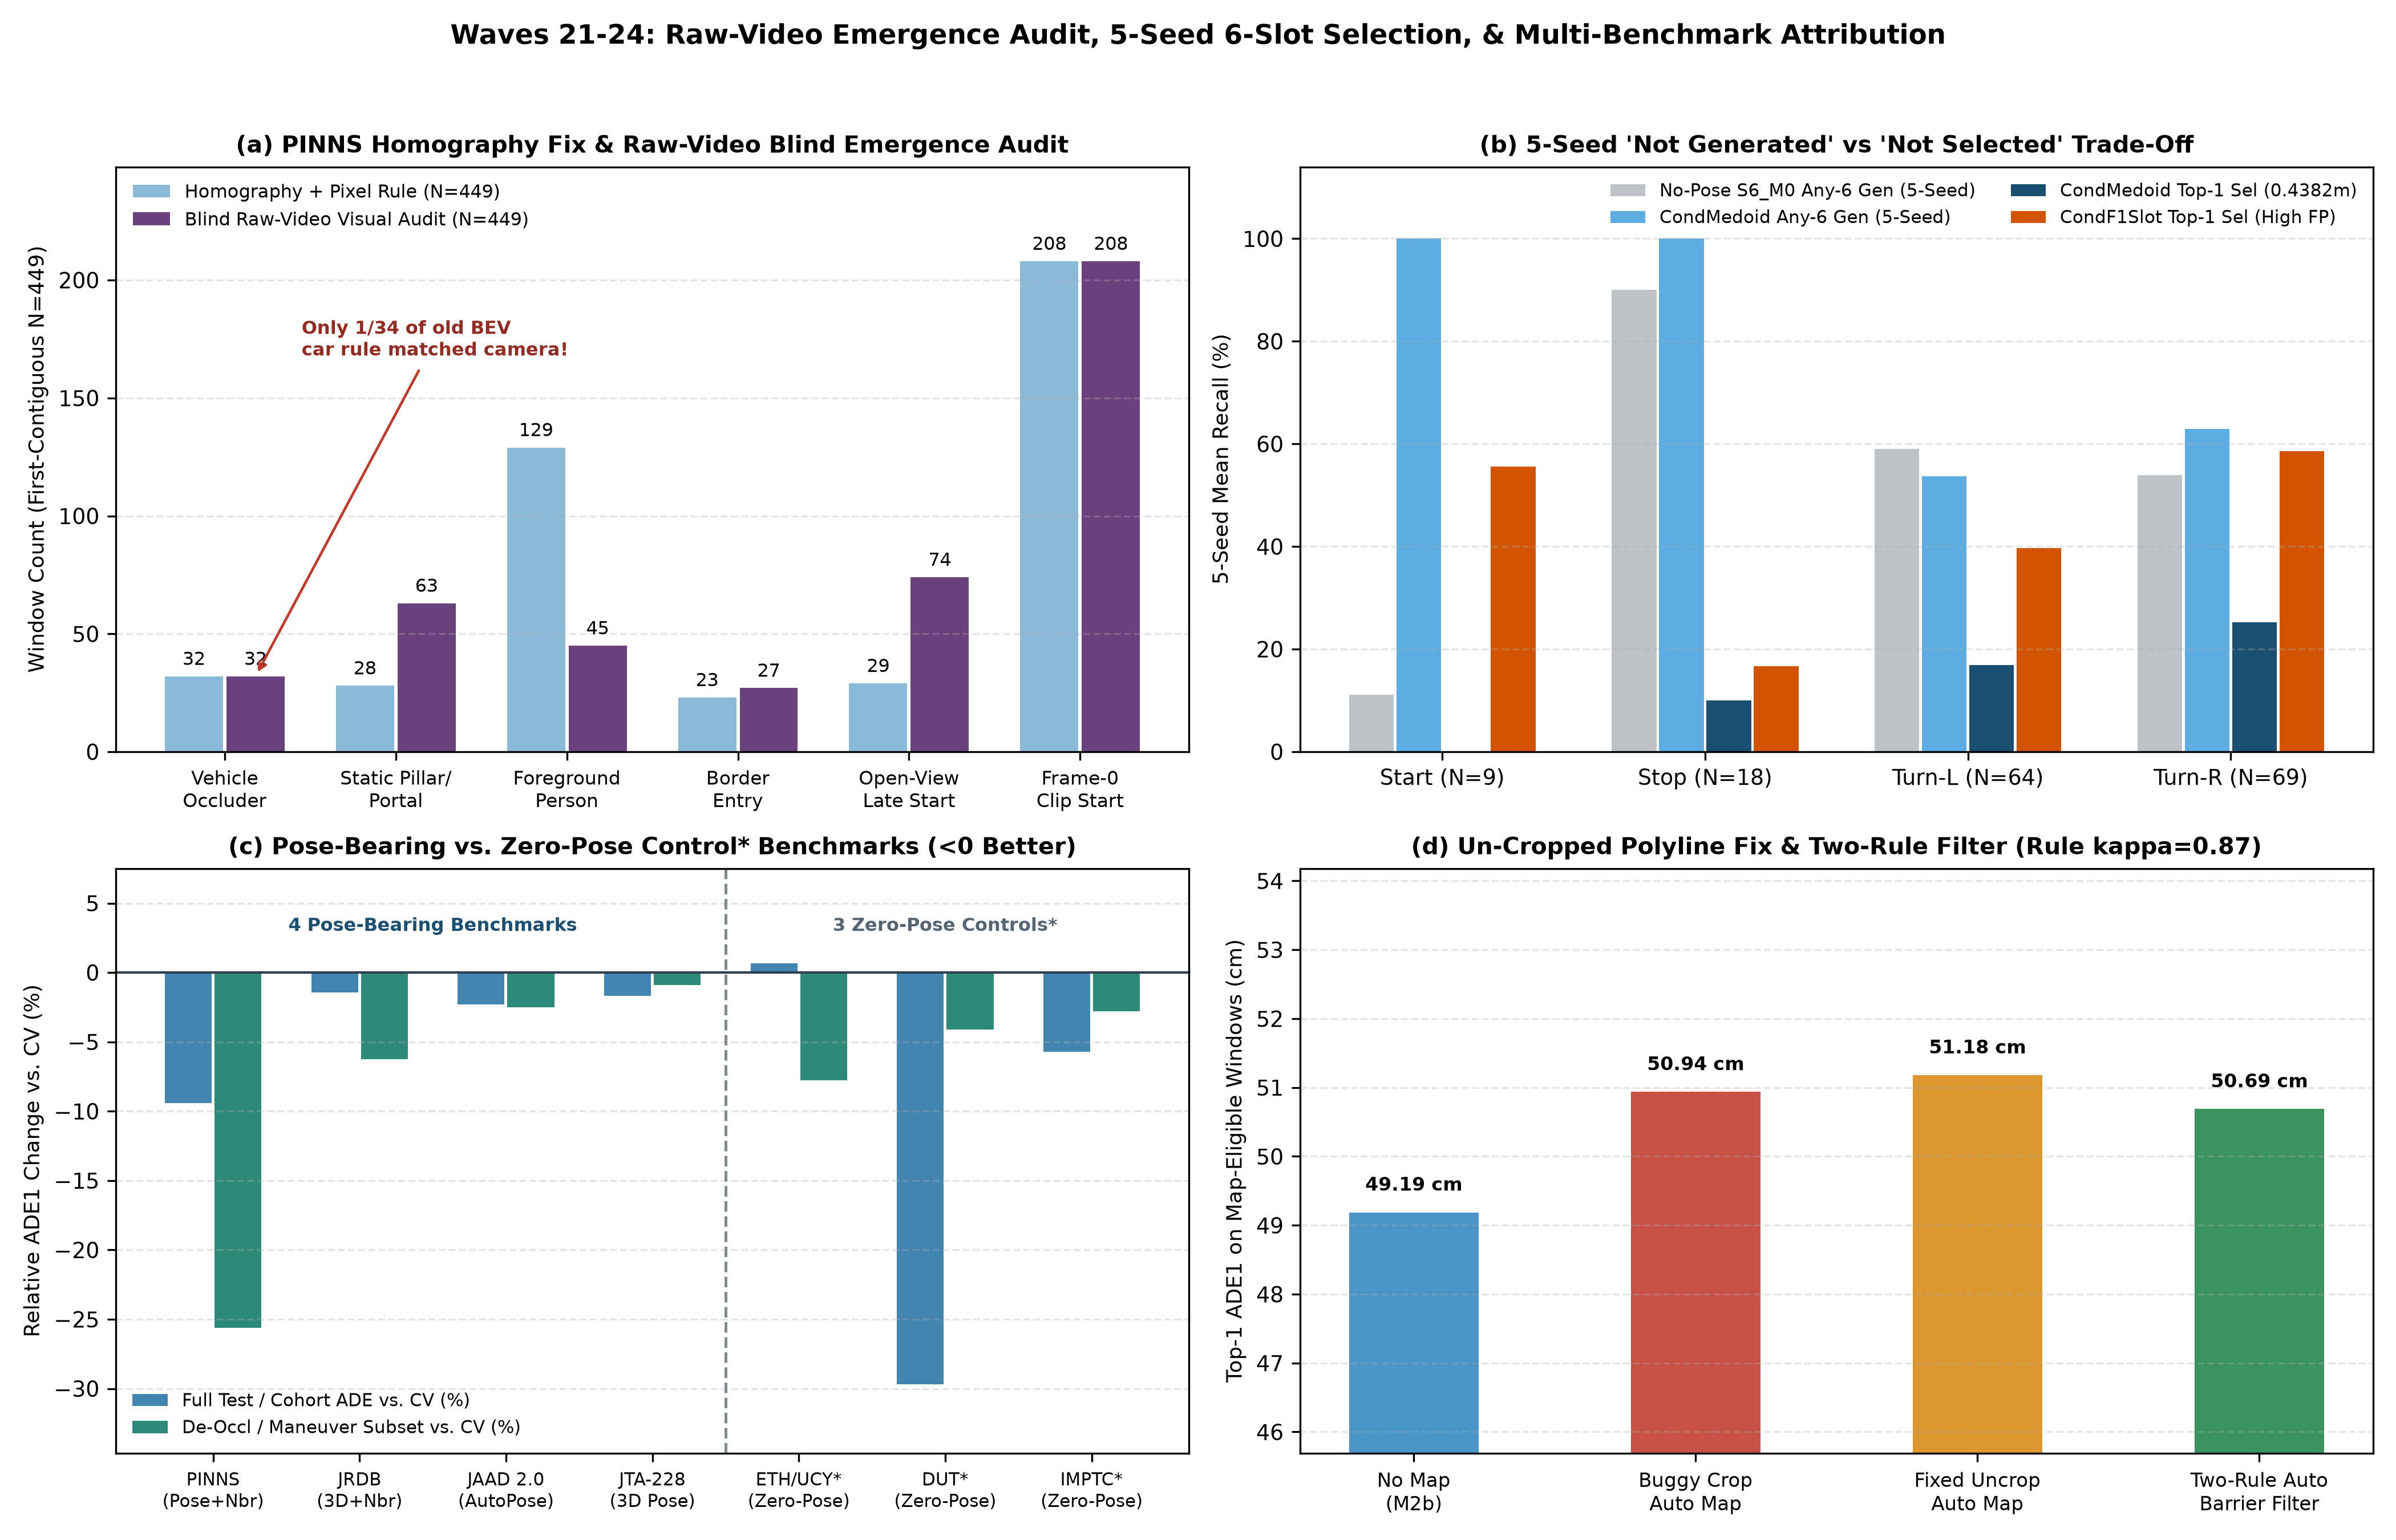
\includegraphics[width=0.95\textwidth]{fig21_wave21_true_emergence_6slot_and_7dataset_precursors.png}
\caption{Prediction-blind raw-video (\texttt{ori\_*.mp4}) emergence decomposition ($140$ visual physical emergences, $208$ Frame-0), 5-seed 6-candidate generation vs.\ Rank-1 selection audit, partitioned pose-bearing vs.\ zero-pose benchmark synthesis, and two-rule automated solid-barrier evaluation ($\kappa_{\text{rule}} = 0.8731$).}
\label{fig:wave21}
\end{figure*}

\begin{figure*}[!t]
\centering
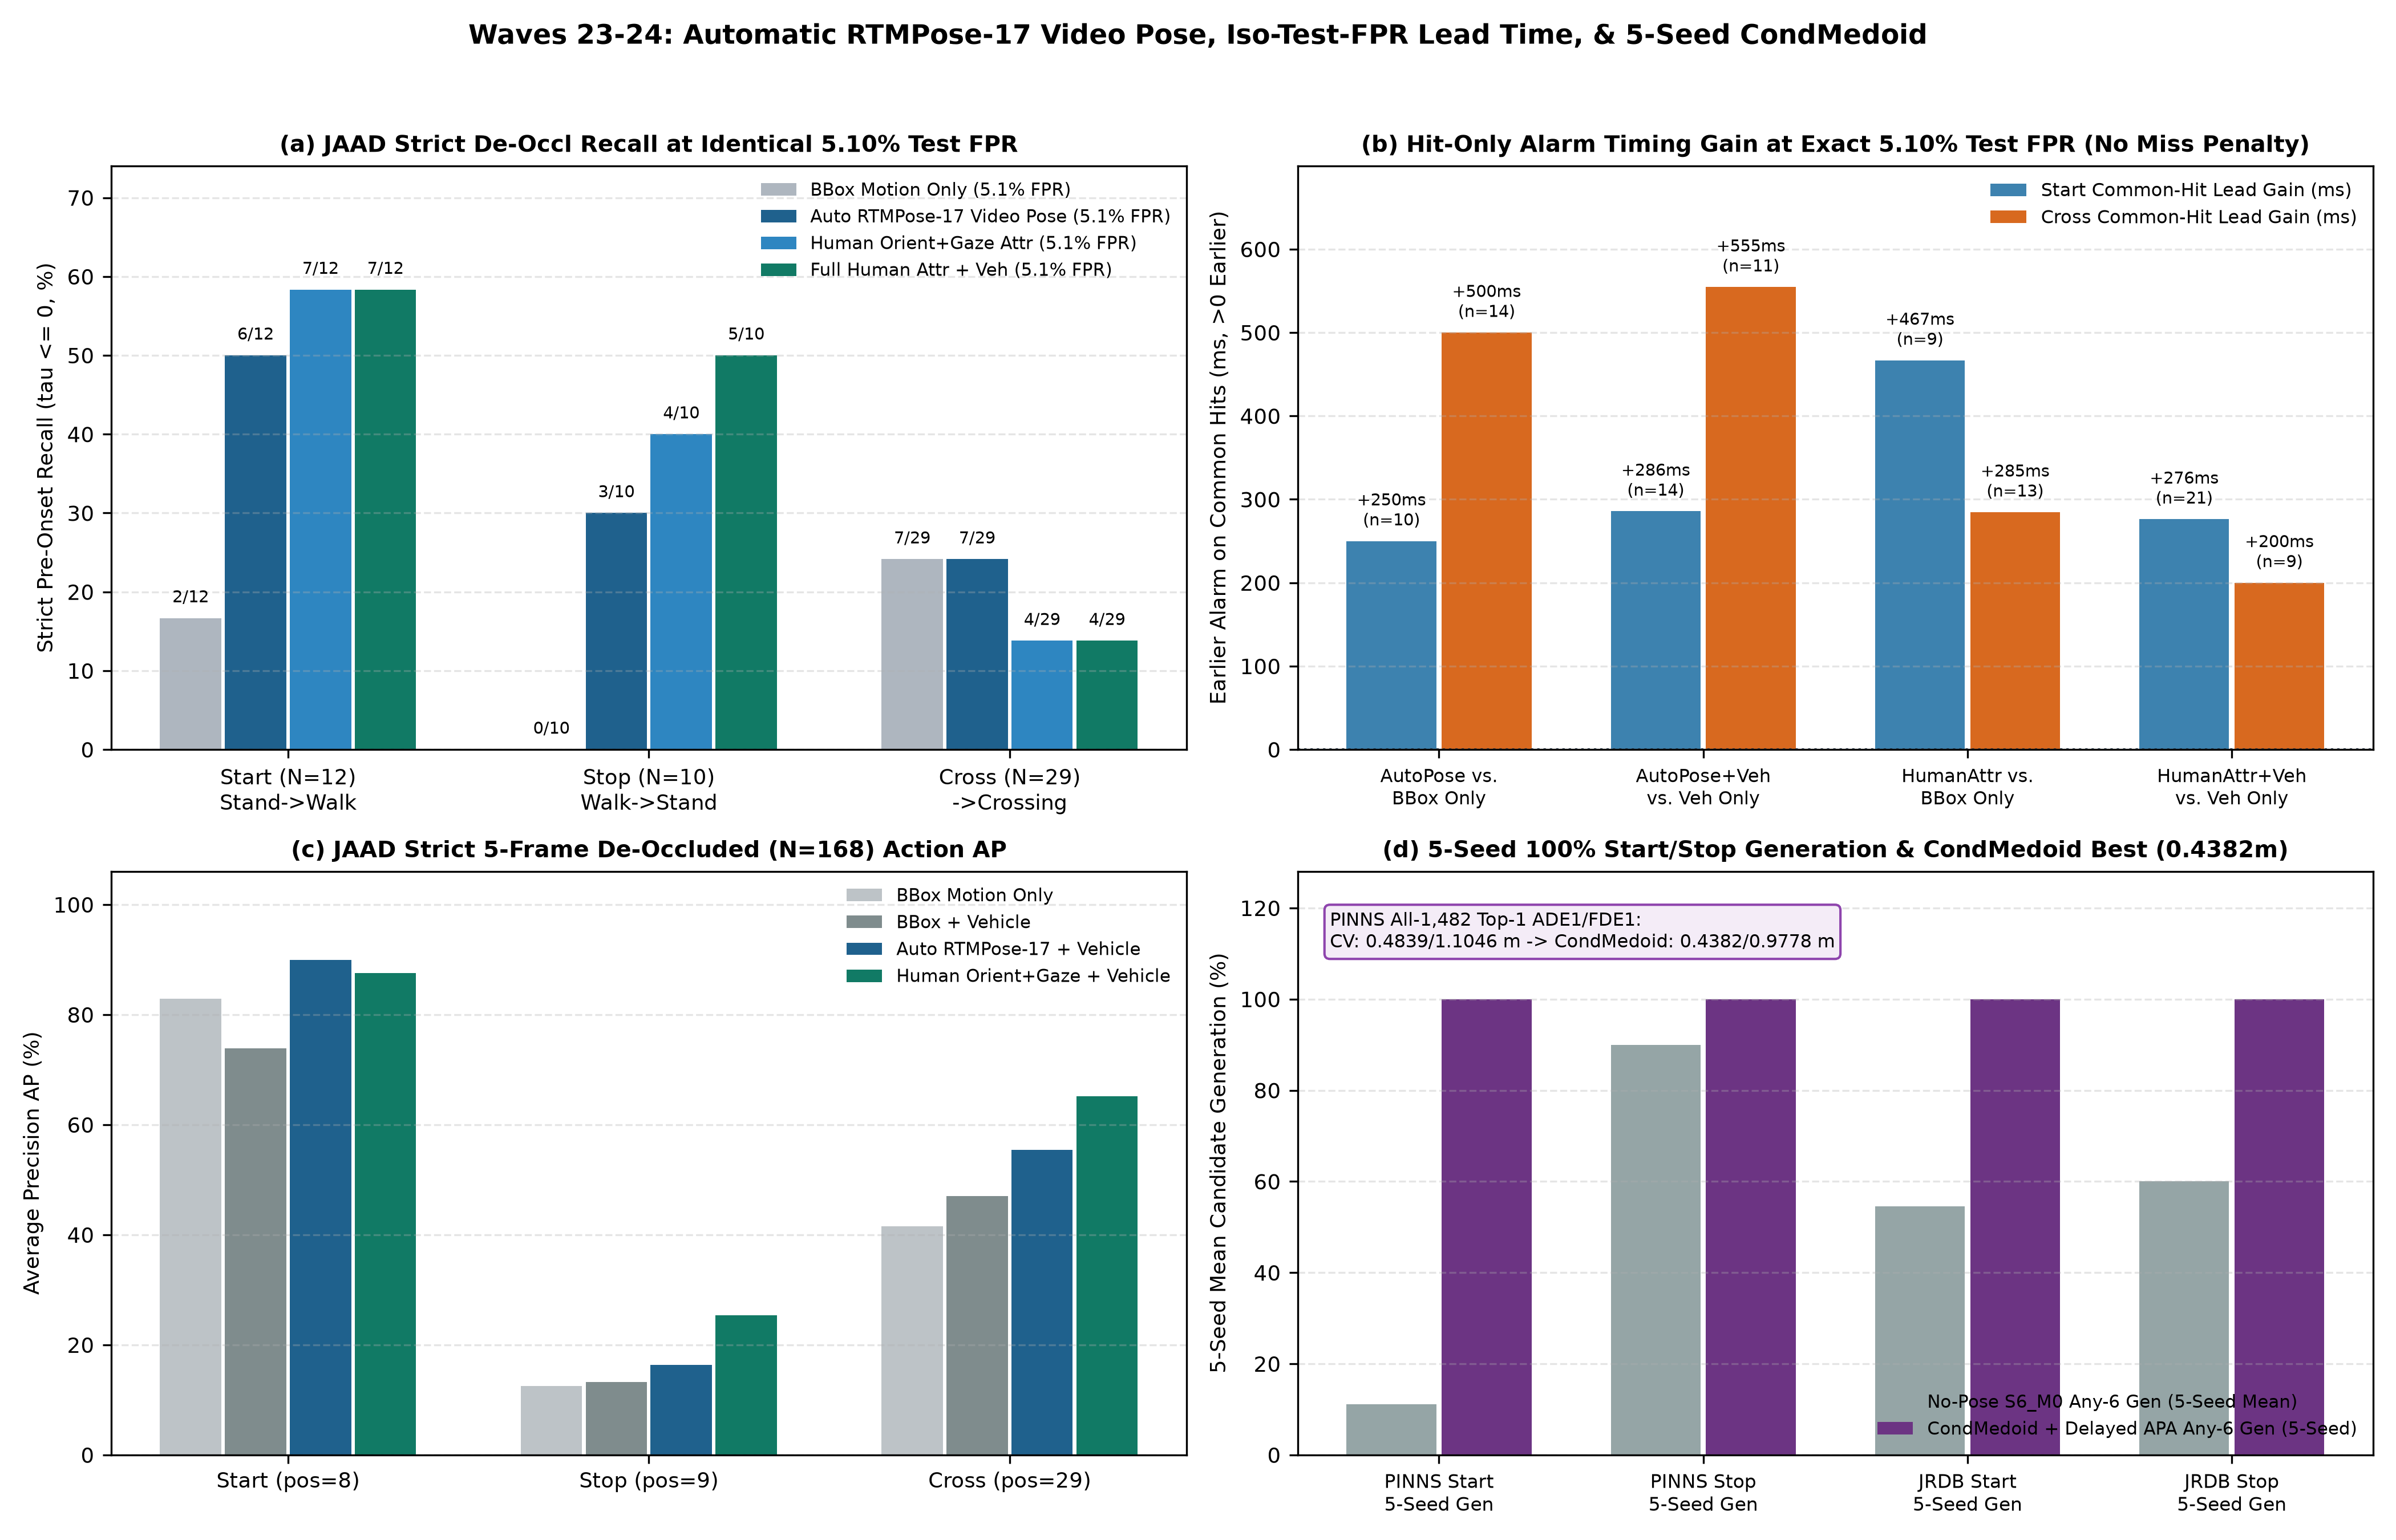
\includegraphics[width=0.95\textwidth]{fig22_wave22_apa_leadtime_and_delayed_onset.png}
\caption{Exact $5.10\%$ realized test-FPR unconflated recall and conditional hit-event alarm timing on strictly de-occluded \texttt{JAAD 2.0} events (\texttt{RTMPose-17} vs.\ \texttt{HumanAttr} vs.\ \texttt{KinOnly}), paired common-hit lead-time delta ($+250.0 / +500.0\text{ ms}$), and 5-seed \texttt{CondMedoid} vs.\ \texttt{CondF1Slot} selection.}
\label{fig:wave22}
\end{figure*}

\section{Discussion, Limitations, and Conclusion}
\textbf{Limitations and Methodological Transparency:} (1) On $<0.5\text{ m}$ monocular emergence (\texttt{first\_short\_323}), single-camera 2D pose back-projection yields $-0.22\text{ cm}$ over \texttt{Regime\_M0} (and $0.3459 / 0.8157\text{ m}$ under \texttt{S6\_Full\_CondMedoid}, $-0.86\text{ cm}$ vs.\ \texttt{Last-2 CV} $0.3545\text{ m}$) yet its 95\% clip CI ($[-2.68, +0.94]\text{ cm}$) remains statistically tied with \texttt{CV}, reflecting $\sim 0.28\text{ m}$ roadside homography tolerances in \texttt{PINNS}~\cite{peng2026pinns} and $54.2\%$ Frame-0 clip-start composition; boxes $<50\text{ px}$ or $q_1 < 0.75$ require monotonic shutoff. (2) Even after un-cropped clip polyline union ($350/835$ windows) and two-rule automated geometric \& causal-trajectory barrier filtering ($\kappa_{\text{rule}} = 0.8731$, $0.27\%$ GT crossing), static $20\text{ m}$ polylines ($0.5069\text{ m}$) do not improve \texttt{Top-1} forecasting over \texttt{No\_Map} ($0.4919\text{ m}$). (3) All $61$ cloud result archives carry dual-layer SHA-256 verification (\url{https://github.com/pjyyyds/Unstructured-ShortPose-Pred}).

\textbf{Conclusion:} Evaluated across four pose-bearing benchmarks and three zero-pose motion/interaction controls, $O(2)$ parity-equivariant Frenet canonicalization, structurally monotonic quality gating, causal radial-conflict neighbor gating, decoupled Platt action reranking, conditioned 6-slot APA medoid selection ($0.4382 / 0.9778\text{ m}$ on \texttt{PINNS}, $0.2764\text{--}0.2786\text{ m}$ surpassing \texttt{CV} on \texttt{JRDB}; real automatic \texttt{RTMPose-17} lifting strict post-de-occlusion \texttt{Start}/\texttt{Stop} recall at exact $5.10\%$ test FPR from $16.7\%/0.0\%$ to $50.0\%/30.0\%$ and firing $+250.0 / +500.0\text{ ms}$ earlier on common \texttt{Start}/\texttt{Cross} hits in \texttt{JAAD 2.0}), and zero-retrain locally-weighted split-conformal calibration deliver compact ($20.7\text{k}\text{--}28.0\text{k}$ parameters), real-time ($2.75\text{--}4.78\text{ ms}$ on \texttt{Tesla T4}), and transparently audited pedestrian forecasting.

\bibliographystyle{IEEEtran}
\bibliography{references}

\end{document}
